%----------------------------------------------------------------------------------------
%	Metropolia Thesis LaTeX Template
%----------------------------------------------------------------------------------------
% License:
% This work is licensed under the Creative Commons Attribution 4.0 International License. To view a copy of this license, visit http://creativecommons.org/licenses/by/4.0/.
%
% Authors:
% Panu Leppäniemi, Patrik Luoto and Patrick Ausderau
%
% Credits:
% Panu Leppäniemi: abstract, def, cleaning,...
% Patrik Luoto: title page, abstract in Finnish, abbreviation, math,...
% Patrick Ausderau: initial version, style, table of content, bibliography, figure, appendix, table, source code listing...
%
% Please:
% If you find mistakes, improve this template and alike, please contribute by sharing your improvements and/or send us your feedback there: https://github.com/panunu/metropolia-thesis-latex
% And of course, if you improve it, add yourself as an author.
%
% Compiler:
% Use XeLaTeX as a compiler.

%----------------------------------------------------------------------------------------
%	THESIS
%----------------------------------------------------------------------------------------

\def\thesislang{finnish} %change this depending on your language
\author{Tomi Haapaniemi}
\def\thesis{Opinnäytetyö/Thesis}
\def\alaotsikko{Alaotsikko/Subtitle}

%Finnish section
\def\otsikko{Hakkuukoneen ajoneuvotietokoneen päivitysmahdollisuudet uudempaan}
\def\tutkinto{Insinööri (AMK)}
\def\kohjelma{Tietotekniikan koulutusohjelma}
\def\suuntautumis{Ohjelmistotekniikka/Sulautettu tietotekniikka}
\def\ohjaajat{
Etunimi Sukunimi, Titteli\newline
Etunimi Sukunimi, Titteli
}
\def\avainsanat{avainsanat}
\def\pvm{\ddmmyyyydate\today}

%English section, for abstract
\title{Possibilities to upgrade embedded computer of Harvester}
\def\metropoliadegree {Bachelor of Engineering}
\def\metropoliadegreeprogramme {Degree Programme in Information Technology}
\def\metropoliaspecialisation {Software Engineering/Embedded Engineering}
\def\metropoliainstructors {
First name Last name, Title (for example: Project Manager)\newline
First name Last name, Title (for example: Principal Lecturer)
}
\def\metropoliakeywords {Keywords}
\date{\today}

%----------------------------------------------------------------------------------------
%	GLOBAL STYLES
%----------------------------------------------------------------------------------------

\documentclass[11pt,a4paper,oneside,article]{memoir}
\usepackage[\thesislang]{babel} 
\usepackage{float}
\usepackage{iflang}
\usepackage{amsmath}
\usepackage{amsfonts}
\usepackage{amssymb}
\usepackage{fontspec}
\usepackage{tocloft}
\usepackage{titlesec}
\usepackage[hyphens]{url}
\usepackage{mathtools}
\usepackage{wallpaper}
\usepackage{datetime}
\usepackage[bookmarksdepth=subsection]{hyperref} % for automagic pdf links for toc, refs, etc.
\usepackage[amssymb]{SIunits}
\usepackage[version=3]{mhchem}
\usepackage{pgfplots} %simple plots etc
\usepackage{pgfplotstable}
\usepackage{tikz} % mindmaps, flowcharts, piecharts, examples at http://www.texample.net/tikz/examples/
\usetikzlibrary{shapes.geometric, arrows}


\renewcommand{\dateseparator}{.}
%condition for adding or not space in TOC
\usepackage{etoolbox}
%for compact list
\usepackage{enumitem}
%for block comment
\usepackage{verbatim}
%for "easier" references
\usepackage{varioref}
%forcing single line spacing in bibliography
\DisemulatePackage{setspace}
\usepackage{setspace}
%including figure (image)
\usepackage{graphicx}
%change the numbering for figure
\usepackage{chngcntr}
%strike trough
\usepackage{ulem}
%euro symbol
\usepackage{eurosym}
%try to count
\usepackage{totcount}
%insert source code
\usepackage{listings}
\usepackage{caption}
\usepackage{color}
%force the width of a table instead of column
\usepackage{tabularx}
\usepackage{booktabs} %why not booktabs? :3

\newcommand\tn[1]{\textnormal{#1}} %use \tn instead of \textnormal
\newcommand\reaction[1]{\begin{equation}\ce{#1}\end{equation}} %\reaction{} for chemical reactions

%NORMAL TEXT
%all text, title, etc. in the same font: Arial
%replace with arial.ttf if you have the fontfile
%NOTE: fontname is case-sensitive
\setmainfont
[BoldFont=LiberationSans-Bold.ttf,
ItalicFont=LiberationSans-Italic.ttf,
BoldItalicFont=LiberationSans-BoldItalic.ttf]
{LiberationSans-Regular.ttf}
%line space
\linespread{1.5}
%\doublespacing
%margin
\usepackage[top=2.5cm, bottom=3cm, left=4cm, right=2cm, nofoot]{geometry}
\setlength{\parindent}{0pt} %first line of paragraph not indented
\setlength{\parskip}{16.5pt} %one empty line to separate paragraph
%list with small line space separation
\tightlists

%IMAGE - FIGURE
%the figures should be placed in the "illustration" folder
\graphicspath{{illustration/}}
%figure number without chapter (1.1, 1.2, 2.1) to (1, 2, 3)
\counterwithout{figure}{chapter}
%border around images
\setlength\fboxsep{0pt}
\setlength\fboxrule{0.5pt}
%caption font size
\captionnamefont{\small}
\captiontitlefont{\small}
%space after figure caption (and other float elements)
\setlength{\belowcaptionskip}{-7pt}

%TABLE
\counterwithout{table}{chapter}

%SOURCE CODE
\definecolor{darkgray}{rgb}{.4,.4,.4}
\definecolor{purple}{rgb}{0.65, 0.12, 0.82}
\lstset{
extendedchars=true,
captionpos=b,
caption=\footnotesize,
basicstyle=\singlespacing\ttfamily,%\small\fontfamily{"Courier"}\selectfont,
keywordstyle=\color{blue}\bfseries,
commentstyle=\color{purple}\itshape,
identifierstyle=\color{black},
stringstyle=\color{red},
showstringspaces=false,
showspaces=false,
numbers=left,
numberstyle=\footnotesize,
numbersep=9pt,
breaklines=true,
tabsize=2,
showtabs=false,
xleftmargin=1cm
}
\IfLanguageName {finnish} {\renewcommand{\lstlistingname}{Listaus}} {} % what is a good translation for this?
%\counterwithout{lstlisting}{chapter}
%moved after begin document, otherwise does not compile

%TOC
%change toc title
\IfLanguageName {finnish} {\addto{\captionsfinnish}{\renewcommand*{\contentsname}{Sisällys}}} {}
%remove dots
\renewcommand*{\cftdotsep}{\cftnodots}
%chapter title and page number not in bold
\renewcommand{\cftchapterfont}{}
\renewcommand{\cftchapterpagefont}{}
%sub section in toc
\setcounter{tocdepth}{2}
%subsection numbered
\setcounter{secnumdepth}{2}
\renewcommand{\tocheadstart}{\vspace*{-15pt}}
\renewcommand{\printtoctitle}[1]{\fontsize{13pt}{13pt}\bfseries #1}
\renewcommand{\aftertoctitle}{\vspace*{-22pt}\afterchaptertitle}
%spacing afer a chapter in toc
\preto\section{%
  \ifnum\value{section}=0\addtocontents{toc}{\vskip11pt}\fi
}
%spacing afer a section in toc
\renewcommand{\cftsectionaftersnumb}{\vspace*{-3pt}}
%spacing afer a subsection in toc
\renewcommand{\cftsubsectionaftersnumb}{\vspace*{-1pt}}
%appendix in toc with "Appendix " + num
\IfLanguageName {finnish} {
  \renewcommand*{\cftappendixname}{Liite\space}
  \renewcommand{\appendixtocname}{Liitteet}
}{\renewcommand*{\cftappendixname}{Appendix\space}}
%appendix header
\IfLanguageName {finnish} {\def\appname{Liite\space}}{\def\appname{Appendix\space}}

%TITLES
%chapter title
\titleformat{\chapter}
{\fontsize{13pt}{13pt}\bfseries\linespread{1}}
{\thechapter}{.5cm}{}
\titlespacing*{\chapter}{0pt}{.32cm}{9pt}
\titleformat{\section}
{\fontsize{12pt}{12pt}\linespread{1}}
{\thesection}{.5cm}{}
\titlespacing*{\section}{0pt}{14pt}{6pt}
\titleformat{\subsection}
{\fontsize{12pt}{12pt}\linespread{1}}
{\thesubsection}{.5cm}{}
\titlespacing*{\subsection}{0pt}{14pt}{6pt}


%QUOTE
\renewenvironment{quote}
  {\list{}{\rightmargin=0pt\leftmargin=1cm\topsep=-10pt}%
  \item\relax\fontsize{10pt}{10pt}\singlespacing}
  {\endlist}

%BIBLIOGRAPHY
%bibliography title to be "references"
\IfLanguageName {finnish} {\addto{\captionsfinnish}{\renewcommand*{\bibname}{Lähteet}}} {\renewcommand\bibname{References}}
\makeatletter %reference list option change
\renewcommand\@biblabel[1]{#1\hspace{1cm}} %from [1] to 1 with 1cm gap
\makeatother %
\setlength{\bibitemsep}{11pt}

%count the appendices (since the chapter counter is reset after \appendix).
%! require to complie 2 times
\regtotcounter{chapter}

%TITLE PAGE
\makeatletter
\renewcommand{\maketitle}{
\thispagestyle{empty}
\ThisCenterWallPaper{1}{viiva}
%
\vspace*{9.5cm}
\tn{\LARGE\@author\\[22pt]\Huge\IfLanguageName {finnish}{\otsikko}{\@title}\\[22pt]\LARGE\alaotsikko\\[1.75cm]}

\parbox{.7\linewidth}{
\IfLanguageName {finnish}{
  Metropolia Ammattikorkeakoulu\\
  \tutkinto \\
  \kohjelma \\
  \thesis\\
  \pvm
} {
  Helsinki Metropolia University of Applied Sciences\\
  \metropoliadegree \\
  \metropoliadegreeprogramme \\
  \thesis\\
  \ddmmyyyydate\today %to be checked date format? 
}
}
\ThisLRCornerWallPaper{1}{metropolia}
%
\clearpage
}
\makeatother

\makepagestyle{tiivis}
\makeevenhead{tiivis}{}{}{Tiivistelmä}
\makeoddhead{tiivis}{}{}{Tiivistelmä}

\makepagestyle{abstract}
\makeevenhead{abstract}{}{}{Abstract}
\makeoddhead{abstract}{}{}{Abstract}

\begin{document}
\counterwithout{lstlisting}{chapter}

%page number always on the top right, clear the "chapter/section" head
\pagestyle{myheadings}
\markright{}
%clear chapter "title" foot page
\makeevenfoot{plain}{}{}{}
\makeoddfoot{plain}{}{}{}

%----------------------------------------------------------------------------------------
%	TITLE PAGE
%----------------------------------------------------------------------------------------

\maketitle
\newpage
\LRCornerWallPaper{1}{footer}

%----------------------------------------------------------------------------------------
%    Tiivistelmä
%----------------------------------------------------------------------------------------

\thispagestyle{tiivis}
\begin{tabular}{ | p{4,7cm} | p{10,3cm} |}
  \hline
  Tekijä(t) \newline
  Otsikko \newline\newline 
  Sivumäärä \newline
  Aika
  & 
  \makeatletter
  \@author \newline 
  \otsikko \newline\newline 
  \makeatother
  \pageref*{LastPage} sivua + \total{chapter} liitettä \newline %! if no appendices, risk to count total of chapter :D
  \pvm		
  \\ \hline
  Tutkinto & \tutkinto
  \\ \hline
  Koulutusohjelma & \kohjelma
  \\ \hline
  Suuntautumisvaihtoehto & \suuntautumis
  \\ \hline
  Ohjaaja(t) & \ohjaajat
  \\ \hline
  \multicolumn{2}{|p{15cm}|}{\begin{singlespacing}\vspace{-22pt}
  Tämä on tiivistelmän ensimmäinen kappale. Tiivistelmän kappaleet loppuvat komentoon newline, jotta saadaan yksi tyhjä rivi aikaiseksi. \newline
  
  Tämä on tiivistlemän toinen kappale.
  \end{singlespacing}} \\[14cm] \hline
  Avainsanat & \avainsanat
  \\ \hline
\end{tabular}
\clearpage

%----------------------------------------------------------------------------------------
%	ABSTRACT
%----------------------------------------------------------------------------------------

\pagestyle{abstract}
\begin{tabular}{ | p{4,7cm} | p{10,3cm} |}
  \hline
  Author(s) \newline
  Title \newline\newline 
  Number of Pages \newline
  Date
  & 
  \makeatletter
  \@author \newline
  \@title \newline\newline
  \pageref*{LastPage} pages + \total{chapter} appendices \newline %! if no appendices, risk to count total of chapter :D
  \IfLanguageName {finnish} {\foreignlanguage{english}{\longdate\@date}} {\@date}
  \makeatother
  \\ \hline
  Degree & \metropoliadegree
  \\ \hline
  Degree Programme & \metropoliadegreeprogramme
  \\ \hline
  Specialisation option & \metropoliaspecialisation
  \\ \hline
  Instructor(s) & \metropoliainstructors
  \\ \hline
  \multicolumn{2}{|p{15cm}|}{\begin{singlespacing}\vspace{-22pt}
  Abstract content
  \end{singlespacing}} \\[14cm] \hline
  Keywords & \metropoliakeywords
  \\ \hline
\end{tabular}
\clearpage

%----------------------------------------------------------------------------------------
%	Acknowledgement ?
%----------------------------------------------------------------------------------------
%\chapter*{Acknowledgement}
%Thanks to my cat
%\clearpage

%----------------------------------------------------------------------------------------
%	TABLE OF CONTENTS
%----------------------------------------------------------------------------------------

\makeevenhead{plain}{}{}{}
\makeoddhead{plain}{}{}{}
\pagestyle{empty} %remove page number in toc (if longer than 2 pages)
\tableofcontents*
\pagestyle{empty} %remove page number in toc (if longer than 1 pages)
\clearpage
\pagestyle{plain}

%list of figure, tables comes here...


%----------------------------------------------------------------------------------------
%    Lyhenteet / Abbreviation
%----------------------------------------------------------------------------------------

\pagestyle{empty}
\setlength{\parskip}{1cm}
\IfLanguageName {finnish} {
  \chapter*{Lyhenteet}
  \cftaddtitleline{toc}{chapter}{Lyhenteet}{}
} {
  \chapter*{Abbreviation}
  \cftaddtitleline{toc}{chapter}{Abbreviation}{}
}
\begin{table}[h]
\setlength{\tabcolsep}{8pt}
\renewcommand{\arraystretch}{2}
\begin{tabular}{l p{12cm}}
x86 & Yleisnimitys Intelin 1987 julkaisemalle CISC-prosessorikäskykannalle. Alkuperäiset 8086/80186/80286 olivat 16-bittisiä, mutta 80386:sta eteenpäin käskykantaa laajennettiin 32-bittiseksi.\\
PS/2 & Sarjaväyläinen, alunperin IBM PS/2 koneessa ollut liitäntäprotokolla, joka yleistyi PC-koneiden standardiliitännäksi näppäimistölle ja hiirelle ennen USB-protokollaa. 5V, GND, data, clock.\\
RS232 & Alunperin v. 1962 esitelty asynkroninen sarjaliitäntäprotokolla, joka oli ennen USB-liitännän yleistymistä yleisin PC-koneiden oheislaitteiden liitäntäväylä.\\
USB & Universal Serial BUS, vuonna 1996 esitelty sarjaväyläinen liitäntä oheislaitteiden liitäntään.\\
IDE/PATA & Integrated Drive Electronics (Parallel AT Attachments), kiintolevyjen ja optisten asemien liittämiseen tarkoitettu 16-bittinen rinnakkainen liitäntäväylä vuodelta 1986.\\
CAN & Controller Area Network, vikasietoinen, differentiaalinen kaksijohtoinen automaatioväylä, jossa liikenne lähetetään priorisoituina sanomina vuodelta 1986\\
%
%OMG & Oh my god\\
%WTF & What the F\\
%TL;DR & Too long, didn't read\\
\end{tabular}
\end{table}

\newpage

%page number always on top right; also for chapter "title" page
\pagestyle{plain}
\makeevenhead{plain}{}{}{\thepage}
\makeoddhead{plain}{}{}{\thepage}

\setcounter{page}{1} %page 1 should be Introduction
\ClearWallPaper
%----------------------------------------------------------------------------------------
%	CONTENT
%----------------------------------------------------------------------------------------

\chapter{Johdanto}

Tietokoneiden käyttöikä on varsinkin vaativissa kohteissa rajallinen.
Kun järjestelmien ikä kasvaa niin varaosien saatavuus vähenee. Viimein
ollaan pisteessä, missä ainoa vaihtoehto on korvata vanha järjestelmä
uudella. Tämä saattaa vaatia mittavia päivitysprojekteja myös
järjestelmää tukeviin kokonaisuuksiin ja vaihdon kannattavuus suhteessa
hyötyyn on huono.

Järjestelmänä on vuonna xxx valmistetun metsätraktori, eli
tuttavallisemmin moto. Motolla on n. yy v käyttöikää jäljellä ja moton
ajoneuvotietokone, jolla hallitaan koneen moottoriasetuksia, että myös
puiden kadon hallintaa, alkaa olemaan elinikänsä loppupäässä.
Alkuperäinen tietokone lakkaa toimimasta kokonaan kuumennettuaan liikaa,
kiintolevy on hajonnyt useaan otteeseen ja akustot alkavat olemaan
uusimisen tarpeessa. Jos laitteiston vaihtaisi kokonaan uudempaan olisi
kyseessä sen verran kallis toimenpide(n. 20 000\euro{}), ettei sitä
kannata tehdä enää kyseiseen metsätraktoriin. Tämän takia tutkimmekin
vaihtoehtoisia ratkaisuita lisätä metsätraktorin käytössä olevalle
tietokonejärjestelmälle elinikää.

Insinöörityön aiheena on löytää hakkuukoneessa olevalle 15v vanhan Sunit
Nero-ajoneuvotietokoneelle korvaava uudempi, mutta ohjelmistoilta ja liitäänöiltä yhteensopiva
tietokone. Tavoitteena on uuden laitteen yhteensopivuus vanhan
kiinnitysjärjestelmän kanssa, liitinyhteensopivuus, sekä ohjelmallisen
tason yhteensopivuus. Aluksi tutustutaan käytössä olevaan laitteistoon
ja sen asettamiin vaatimuksiin. Seuraavaksi käydään läpi mahdollisia
toteuttamisvaihtoehtoja ja niiden ominaisuuksia. Asennetaan uusi
ohjelmisto testikannetavaan ja testataan järjestelmä
tuotantoympäristössä. Lopuksi tutkitaan mahdolliset

Haasteita työlle asettavat vanhat ohjelmistot, tärinää ja pölyä ja
vaihtelevia lämpötiloja sisältävä työympäristö. Metsätraktori on
huoltoja lukuunottamatta metsässä kesät talvet ja lämpötilat vaihtelevat
talvella -20 asteesta +20 asteeseen ja kesäisin lämmöt voivat nousta
ohjaamossa jopa +50-60 asteeseen.

\section{Standardeja}

\subsection{EU-direktiivi 2004/104/EY}

Direktiivi 2004/104/EY (Autoteollisuuden EMC-direktiivi) määrittää, että
1.7.2006 alkaen valmistettujen ajoneuvojen ja kiinteiästi asennetun
ajoneuvoelektroniikan aiheuttamat säteilypäästöt ja päästöjen sietokyky
mitataan kyseisen direktiivin mukaisesti. Direktiiviin on julkaistu
lisäys 2005/83/EY, joka tarkentaa direktiiviä. Uusi direktiivi korvaan
aiemman direktiivin 95/54/EY.

Uusi direktiivi vaatii tyyppihyväksynnän vain laitteilta, joilla on
vaikutusta ajoneuvon hallintaan, kuljettajan asennon muuttamiseen tai
kuljettajan näkyvyysalueeseen. Laitteiden, joiden ei tarvitse olla
tyyppihyväksyttyjä, pitää täyttää kuitenkin EMC-direktiivin 89/336/ETY
tai radio- ja telepäätelaitedirektiivin 1999/5/EY vaatimukset. (S. Oy
2006) \cite{1999/5/EY} \cite{89/336/ETY}

\subsection{EMC-direktiivi 89/336/ETY ja
2004/108/EY}

EMC-direktiivi 89/336/ETY määrittelee ainoastaan laitteistolta
vaadittavat ominaisuudet sähkömagneettisen yhteensopivuuden
takaamiseksi. Direktiivin tarkoitus on ohjeistaa valmistajia tekemään
elektromagneettisesti yhteensopivia laitteita. Direktiivi koskee kaikkia
sähkölaitteita ja -asennuksia, joita ei direktiivissä ole erikseen
rajattu sen ulkopuolelle \cite{89/336/ETY}. Direktiivi 2004/108/EY
kumosi vanhemman direktiivin 89/336/ETY 20.7.2004 alkaen. 2004/108/EY
mm. erotteli kiinteille asennuksille ja laitteille tehtävät asennukset,
sekä yksinkertaisti vaatimustenmukaisuuden arviointimenettelyä.
\cite{2004/108/EY}

\subsection{Radio- ja telepäätelaitedirektiivi
1999/5/EY}

Radio- ja telepäätelaitedirektiivi 1999/5/EY määrittää radio ja
telepäätelaitteiden yhteensopivuuden euroopan laajuisesti. Kaikkiin
direktiivin piiriin kuuluvien laitteiden tulee olla turvallisia
käyttäjälle ja muille henkilöille, sekä täyttää vaaditut
suojavaatimukset sähkömagneettisen yhteensopivuuden osalta. Lisäksi
direktiivi määrittää että laitteistojen tulee olla rakennettuja siten
että ne käyttävät tehokaasti radioviestintään varattua spektriä ja
resursseja. Tietyille laiteluokille on lisäksi määritelty vielä muita
vaadittuja lisäominaisuuksia, kuten yksityisyyden suojan takaamisen,
yhteensopivuuden muiden laitteistojen välillä, sisältävät petoksia
ehkäiseviä ominaisuuksia, tukevat hätäpalveluihin pääsyn takaavia
ominaisuuksia ja/tai sisältävät ominaisuuksia joilla laitteistojen
käyttö tehdään helpommaksi vammaisille {[}@1999/5/EY{]}. Direktiivi
1999/5/EY on kumottu 13.6.2016 alkaen direktiivillä 2014/53/EU
radiolaitteiden asettamista saataville markkinoilla koskevan
jäsenvaltioiden lainsäädännön yhdenmukaistamisesta. {[}@2014/53/EU{]}

\subsection{IP-suojaluokitus}

IP-suojaluokitus on standardissa IEC 60529 määritetty järjestelmä
sähkölaitteiden tiiveyden määrittämiseksi. IP-luokitus kertoo laitteiden
suojauksen pölyä ja vettä vastaan. \cite{IEC60529}

\subsubsection{IP54}

IP54-suojaluokitetut tuotteet ovat pölysuojattuja (ei täydellistä
tiiveyttä, mutta ei pölykertymiä), sekä roiskesuojattuja.

\subsubsection{IP67/66}

IP67/66 -suojaluokitetut tuotteet ovat täysin pölytiiviitä ja kestävät
suurella paineella tulevan vesiruiskun. IP67/66-tuotteet kestävät
tärinää ja iskuja 5M3-vaatimusten mukaisesti. (DIN EN 60721-3-5, MIL-STD
810F.)

\chapter{Taustaa}
\section{Hakkuukoneet}

Hakkuukoneet eli motot (monitoimikoneet) ovat metsätraktoreita, joiden
tehtävänä on hakkuun kaikki työvaiheet. Hakkuukoneet sisältävät
tietokoneohjatut mittalaitteet joilla puiden katkonta ja mittaus saadaan
hoidettua tarkasti.

\subsection{Hakkuukone Valmet xxx}

Lorem ipsum dolor sit amet, consectetur adipiscing elit. Nam sed gravida
ex. Sed leo nisl, viverra in efficitur eget, imperdiet vel nibh. Donec
gravida sapien facilisis nisl rhoncus, sit amet ullamcorper nulla
congue. Donec egestas nisi sed finibus tempus. Integer convallis
suscipit magna et sollicitudin. Fusce gravida nisl eros, sit amet congue
odio aliquam vel. Vivamus congue massa eget est efficitur, dapibus
lacinia velit porttitor. Nunc consectetur sit amet augue vel ultrices.
Nullam hendrerit nisi efficitur tincidunt molestie.

\subsection{Motomit-mittalaite}

Kohteena olevaan Valmet xxx-hakkuukoneeseen on jälkiasennettu Motomit-IT
-mittalaite, joka on korvannut hakkuukoneen alkuperäiset mittalaitteet
ja ohjelmiston hakkuussa. Motomit IT tukee StanForD-standardin mukaista
apteerausohjeiden tiedonsiirtoa. Motomit IT hoitaa sisäisen
kommunikaation CAN-väylää pitkin. Kommunikaatiossa alkuperäisen
ajoneuvotietokoneen kanssa käytetään RS232-väylää ja MotomitPC
-ohjelmistoa. (P. L. Oy 2008)

\begin{figure}[H]
\centering
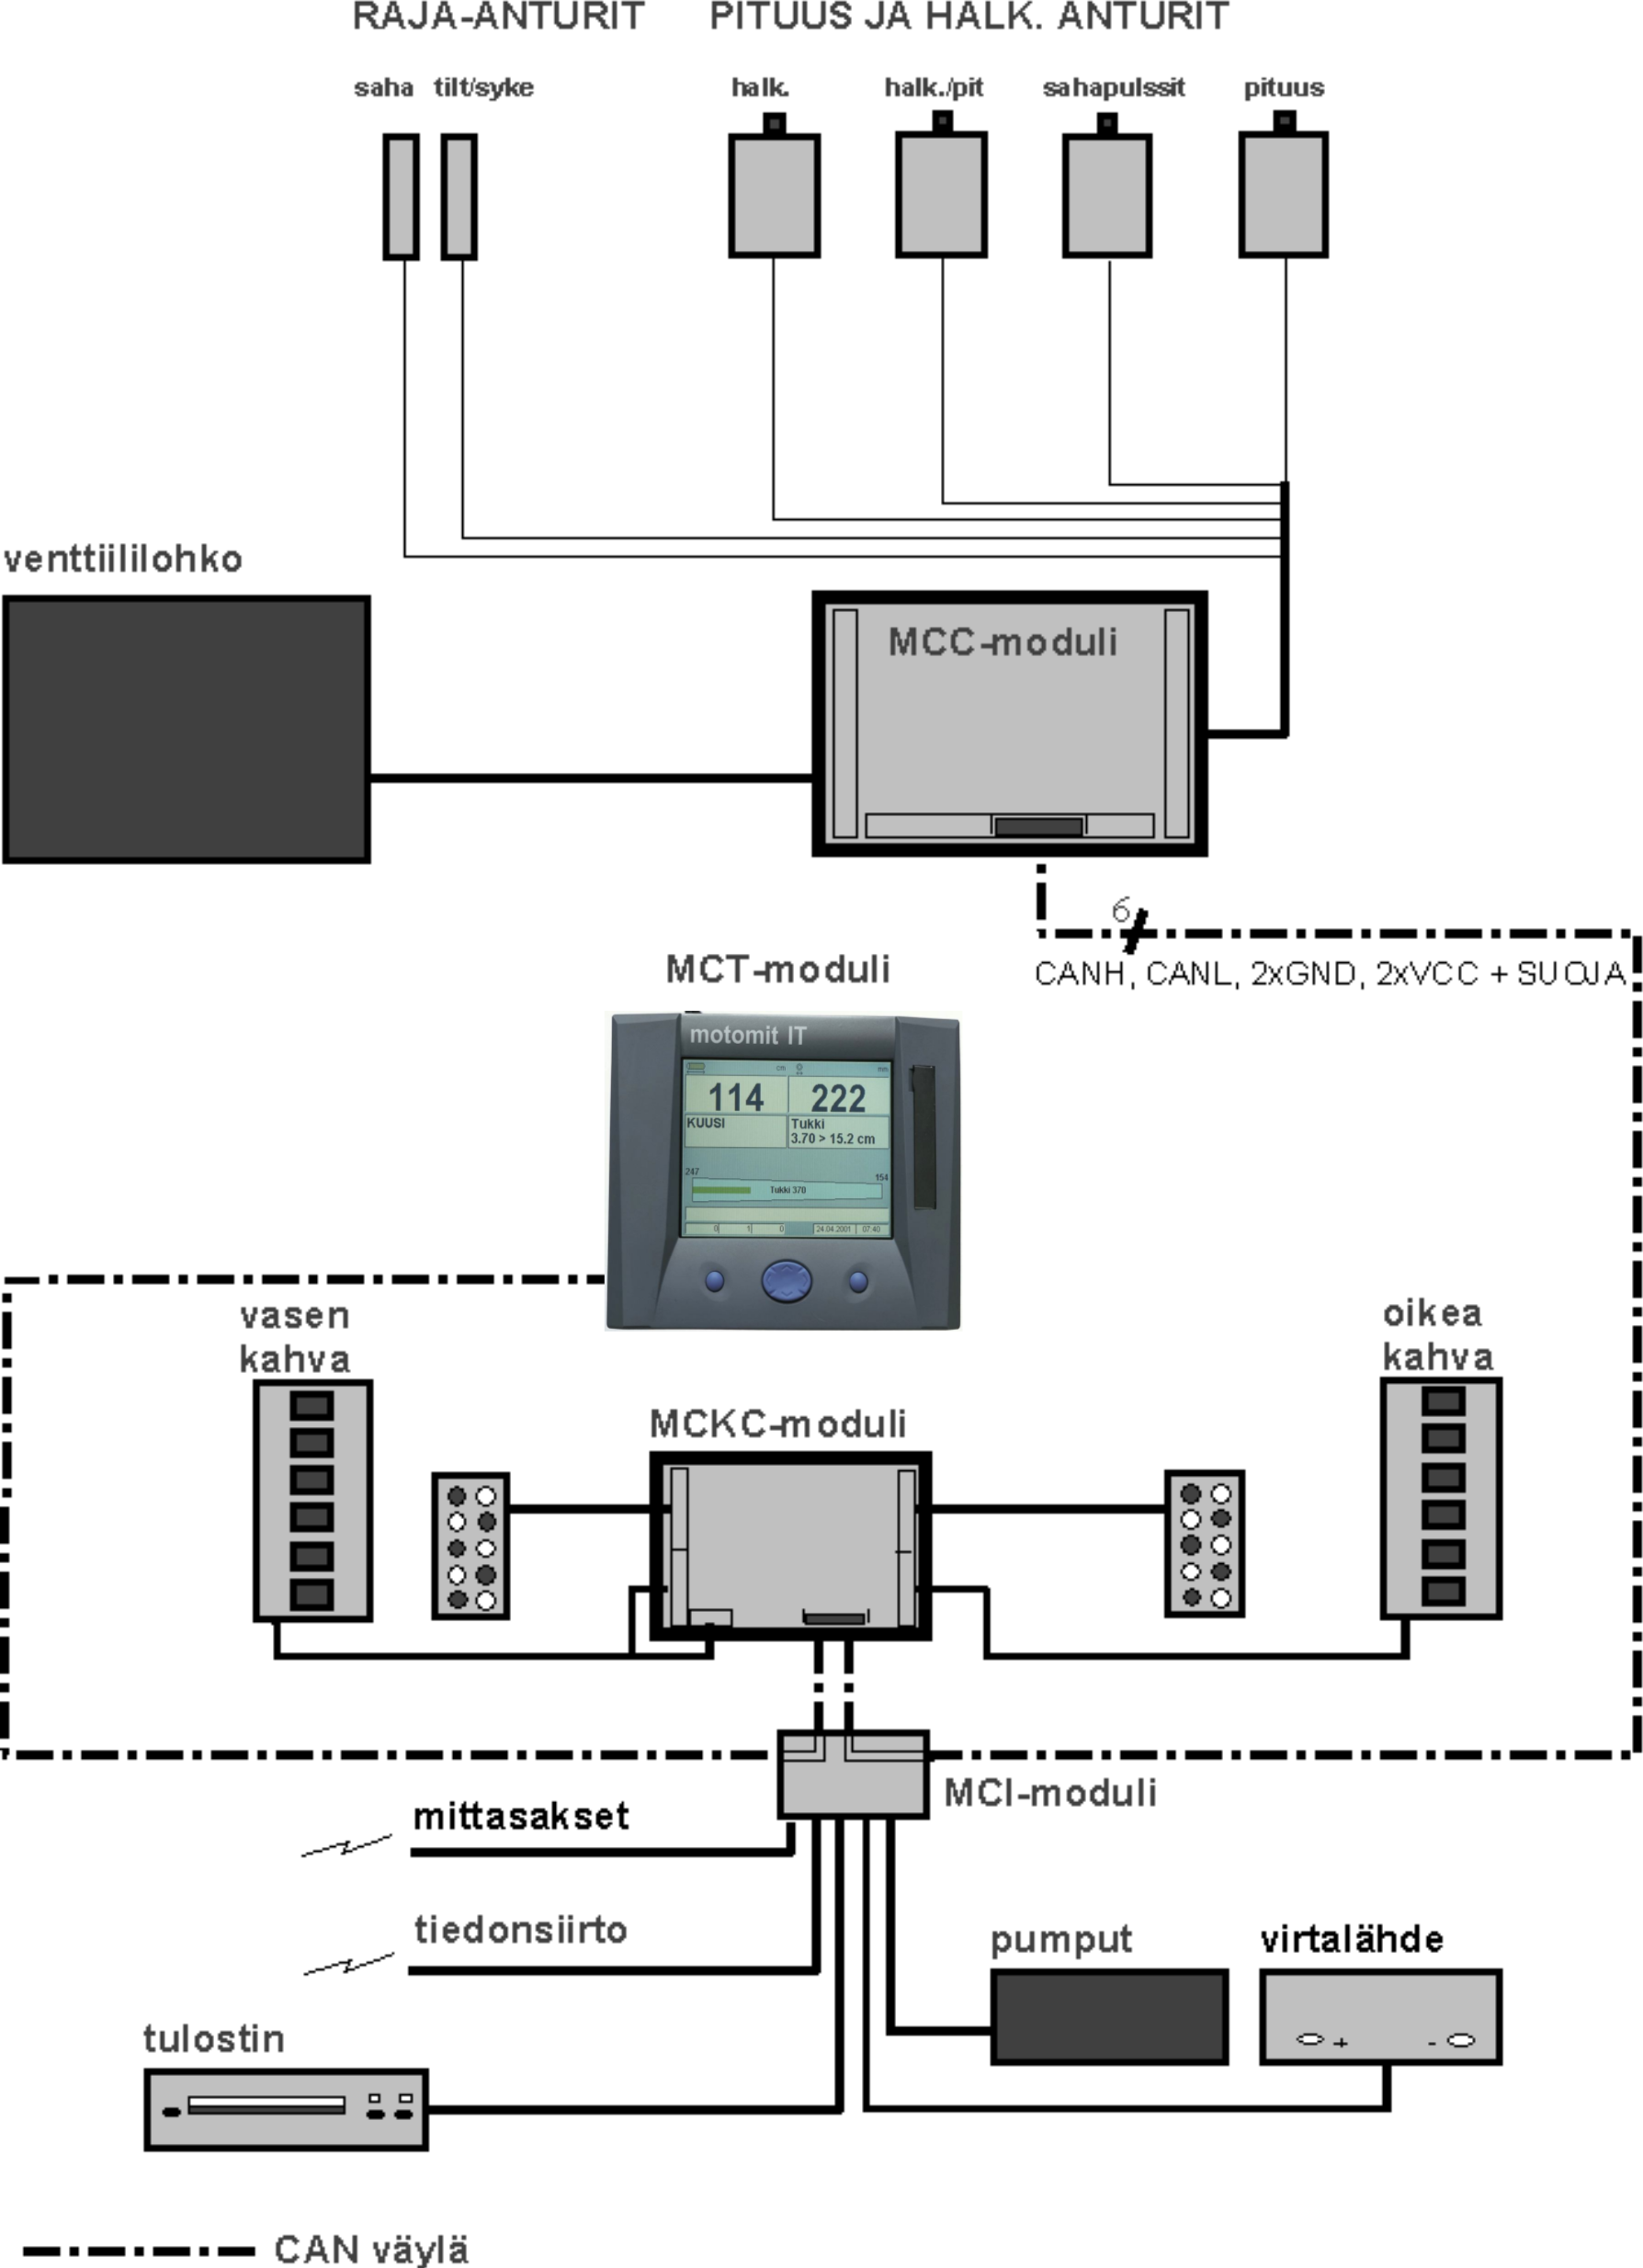
\includegraphics[width=1.000\textwidth]{/home/th/repos/motonkone/pictures/motomit_kaavio.png}
\caption{Motomit IT:n moduulikaavio}
\end{figure}

\section{Alkuperäinen PC-järjestelmä}

\subsection{Ajoneuvo-PC Sunit Nero / Valmet Maxi}

Hakkuukoneessa käytetty tietokone on Sunitin valmistama Sunit Nero (myös nimellä Valmet MAXI)-ajoneuvotietokone. Nero on paketoitu näyttöineen ja keskusyksikköineen yhdeksi all-in-one -tyyliseksi iskunkestäväksi paketiksi. Vaikka kyseessä ei olekaan sama yksilö mikä on alunperin ollut kiinni kyseisessä hakkuukoneeessa, on se samanlainen kuin alkuperäinen ja samaa ikäluokkaa (n. 17v, vuodelta 1997? ). Emolevyn northbridge-ohjaimena on SiS 5571-ohjain. Tässä Nero-yksilössä prosessorina on AMD:n 300 MHz Socket 7-kantainen K6-prosessori vuodelta 1998 (alkuperäinen prosessori on vaihdettu useita vuosia sitten tehdyn huollon yhteydessä toiseen), 64 Mb keskusmuistia. Tietokoneen kiintolevynä oli tutkintahetkellä Western Digitalin 120 Gb:n Scorpio Blue-kiintolevy, joka sekin on vaihdettu kyseiseen yksilöön useaan kertaan. Nero-tietokoneesta löytyy 3,5" levykseasema, sekä cd-asema. Näyttöpaneeli on 4:3-kuvasuhteella ja 800x600 pikselin resoluutiolla oleva 12" LCD-paneeli. Koneessa on lisäksi NiMH-akku BIOSin asetusten säilyttämiseen. Tietokoneesta löytyy liitännät sekä 12V ja 24V jännitteille. Sunitin huolto on ilmoittanut, etteivät he suostu/pysty enää huoltamaan näin vanhaa tietokonetta.

\begin{figure}[H]
\centering
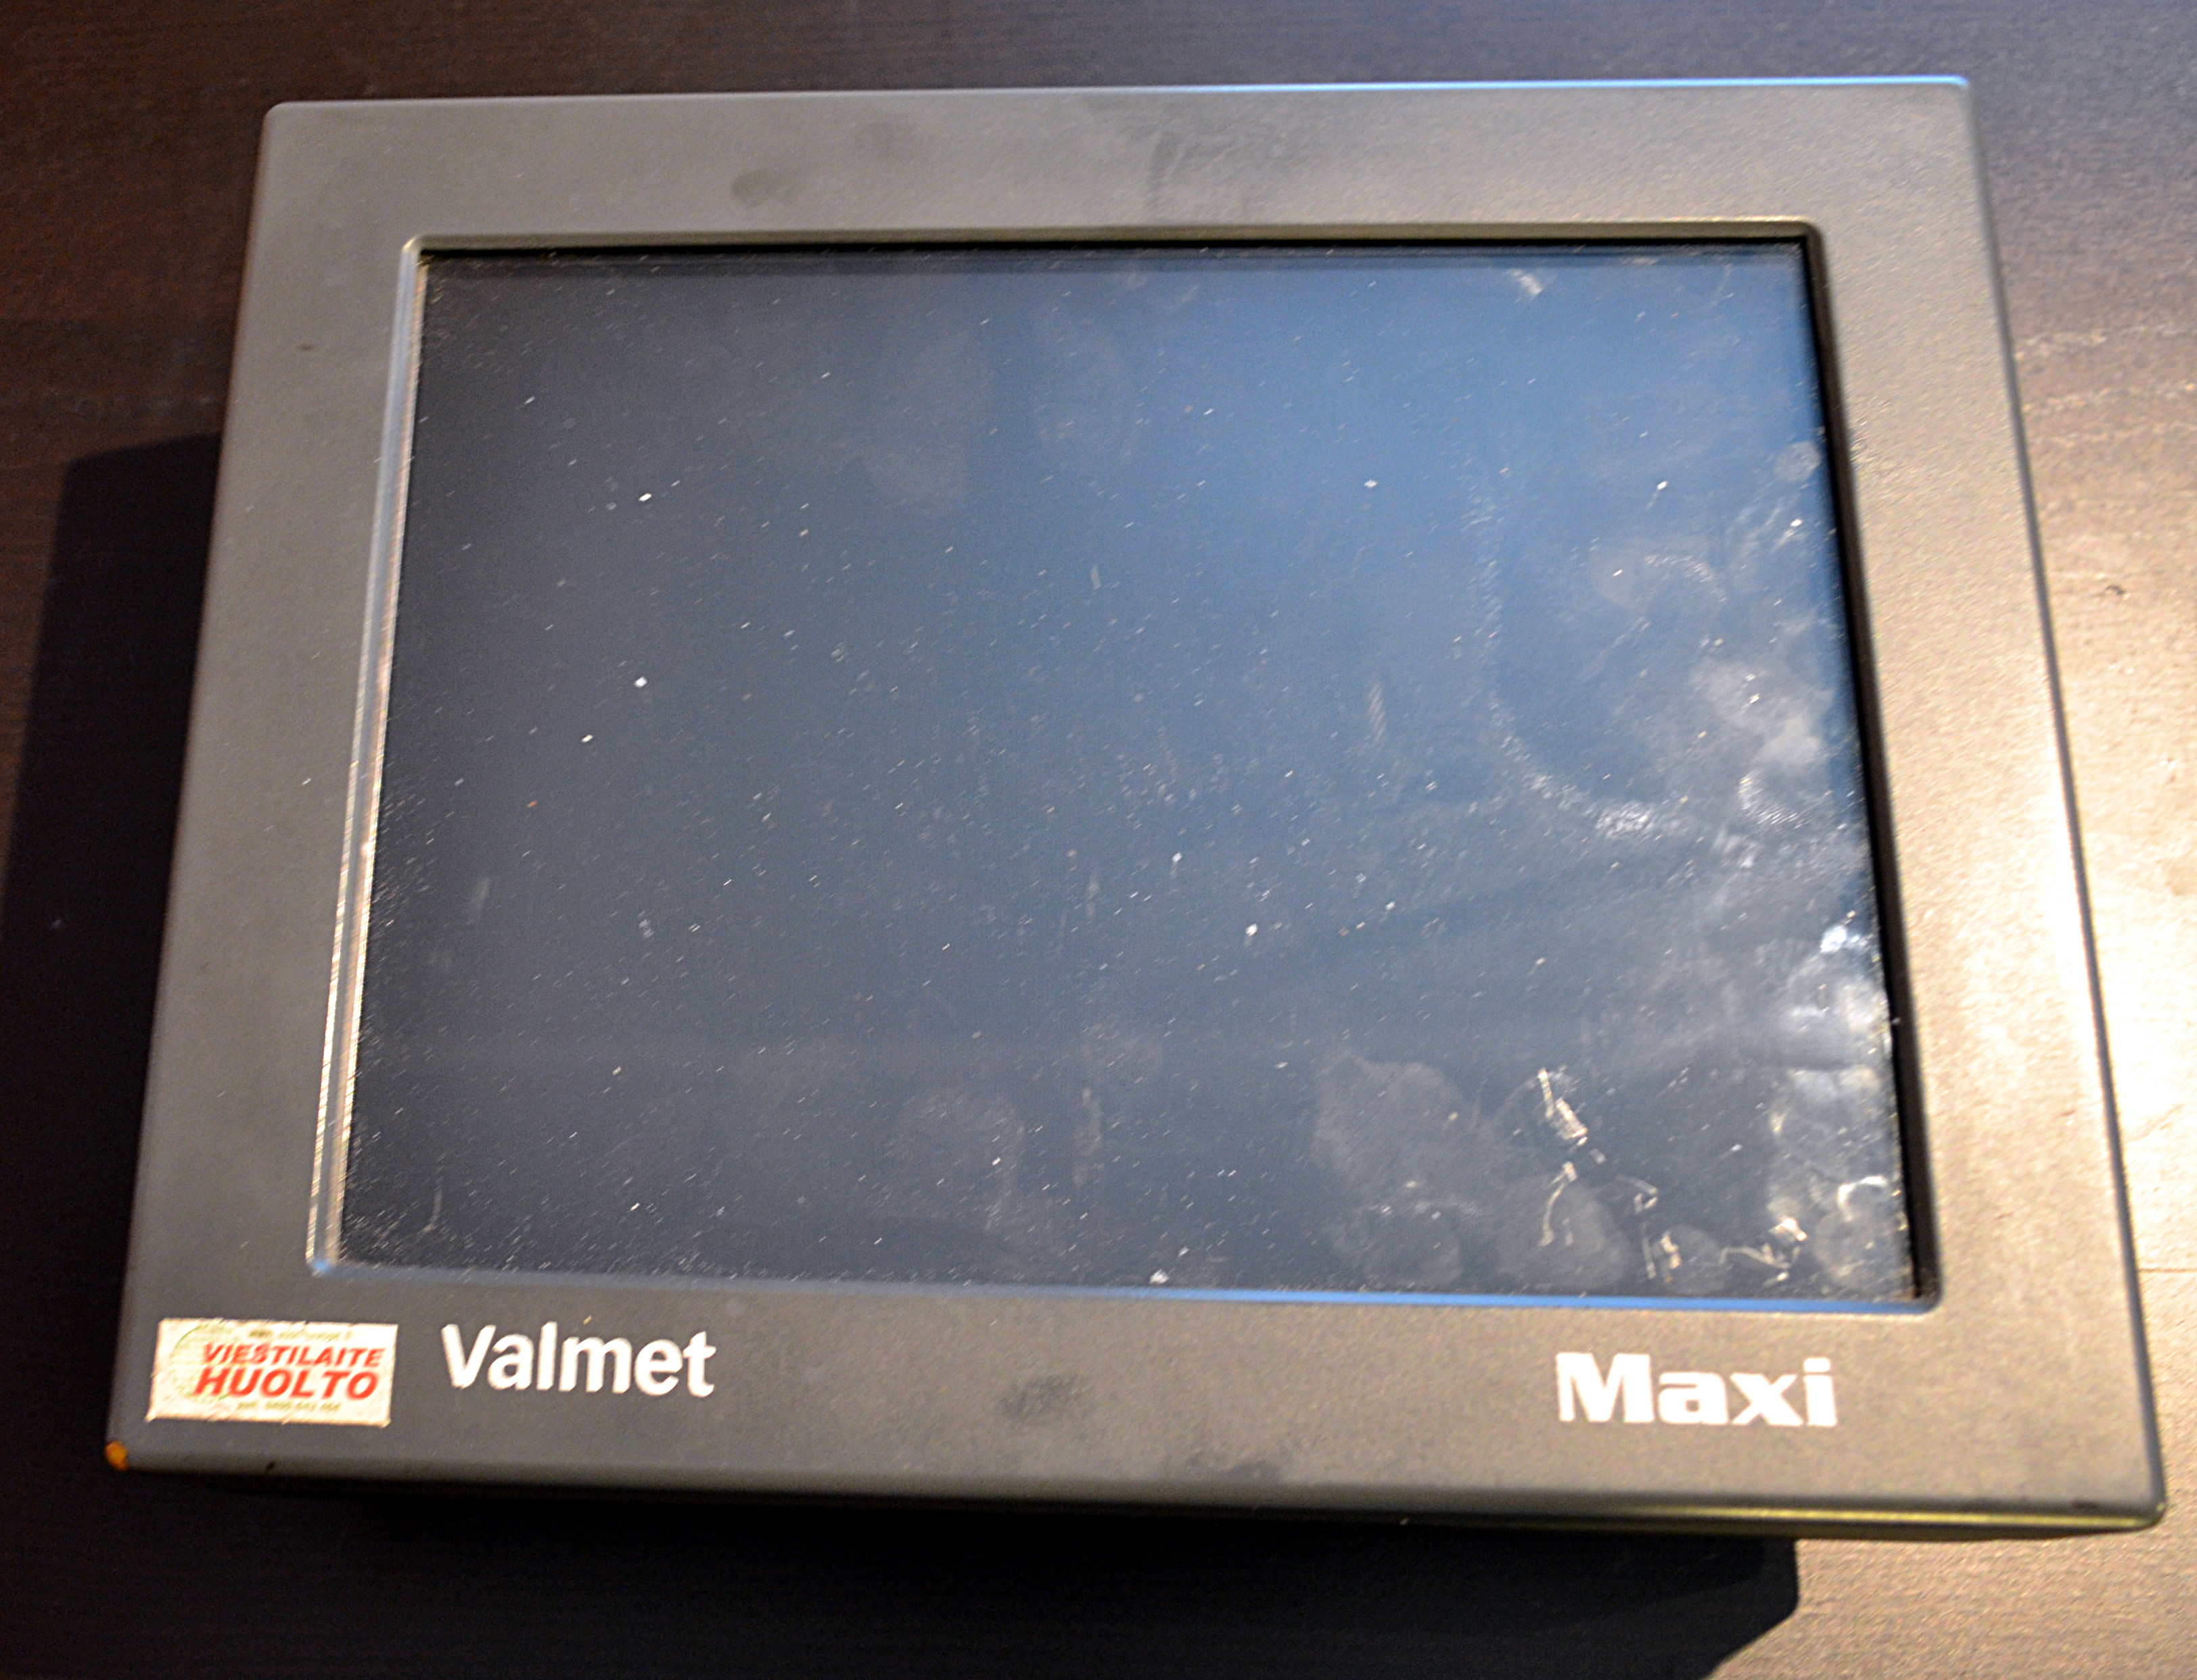
\includegraphics[width=1.000\hsize]{/home/th/repos/motonkone/pictures/valmet_maxi.jpg}
\caption{Sunit Nero / Valmet Maxi}
\end{figure}

\begin{figure}[H]
\centering
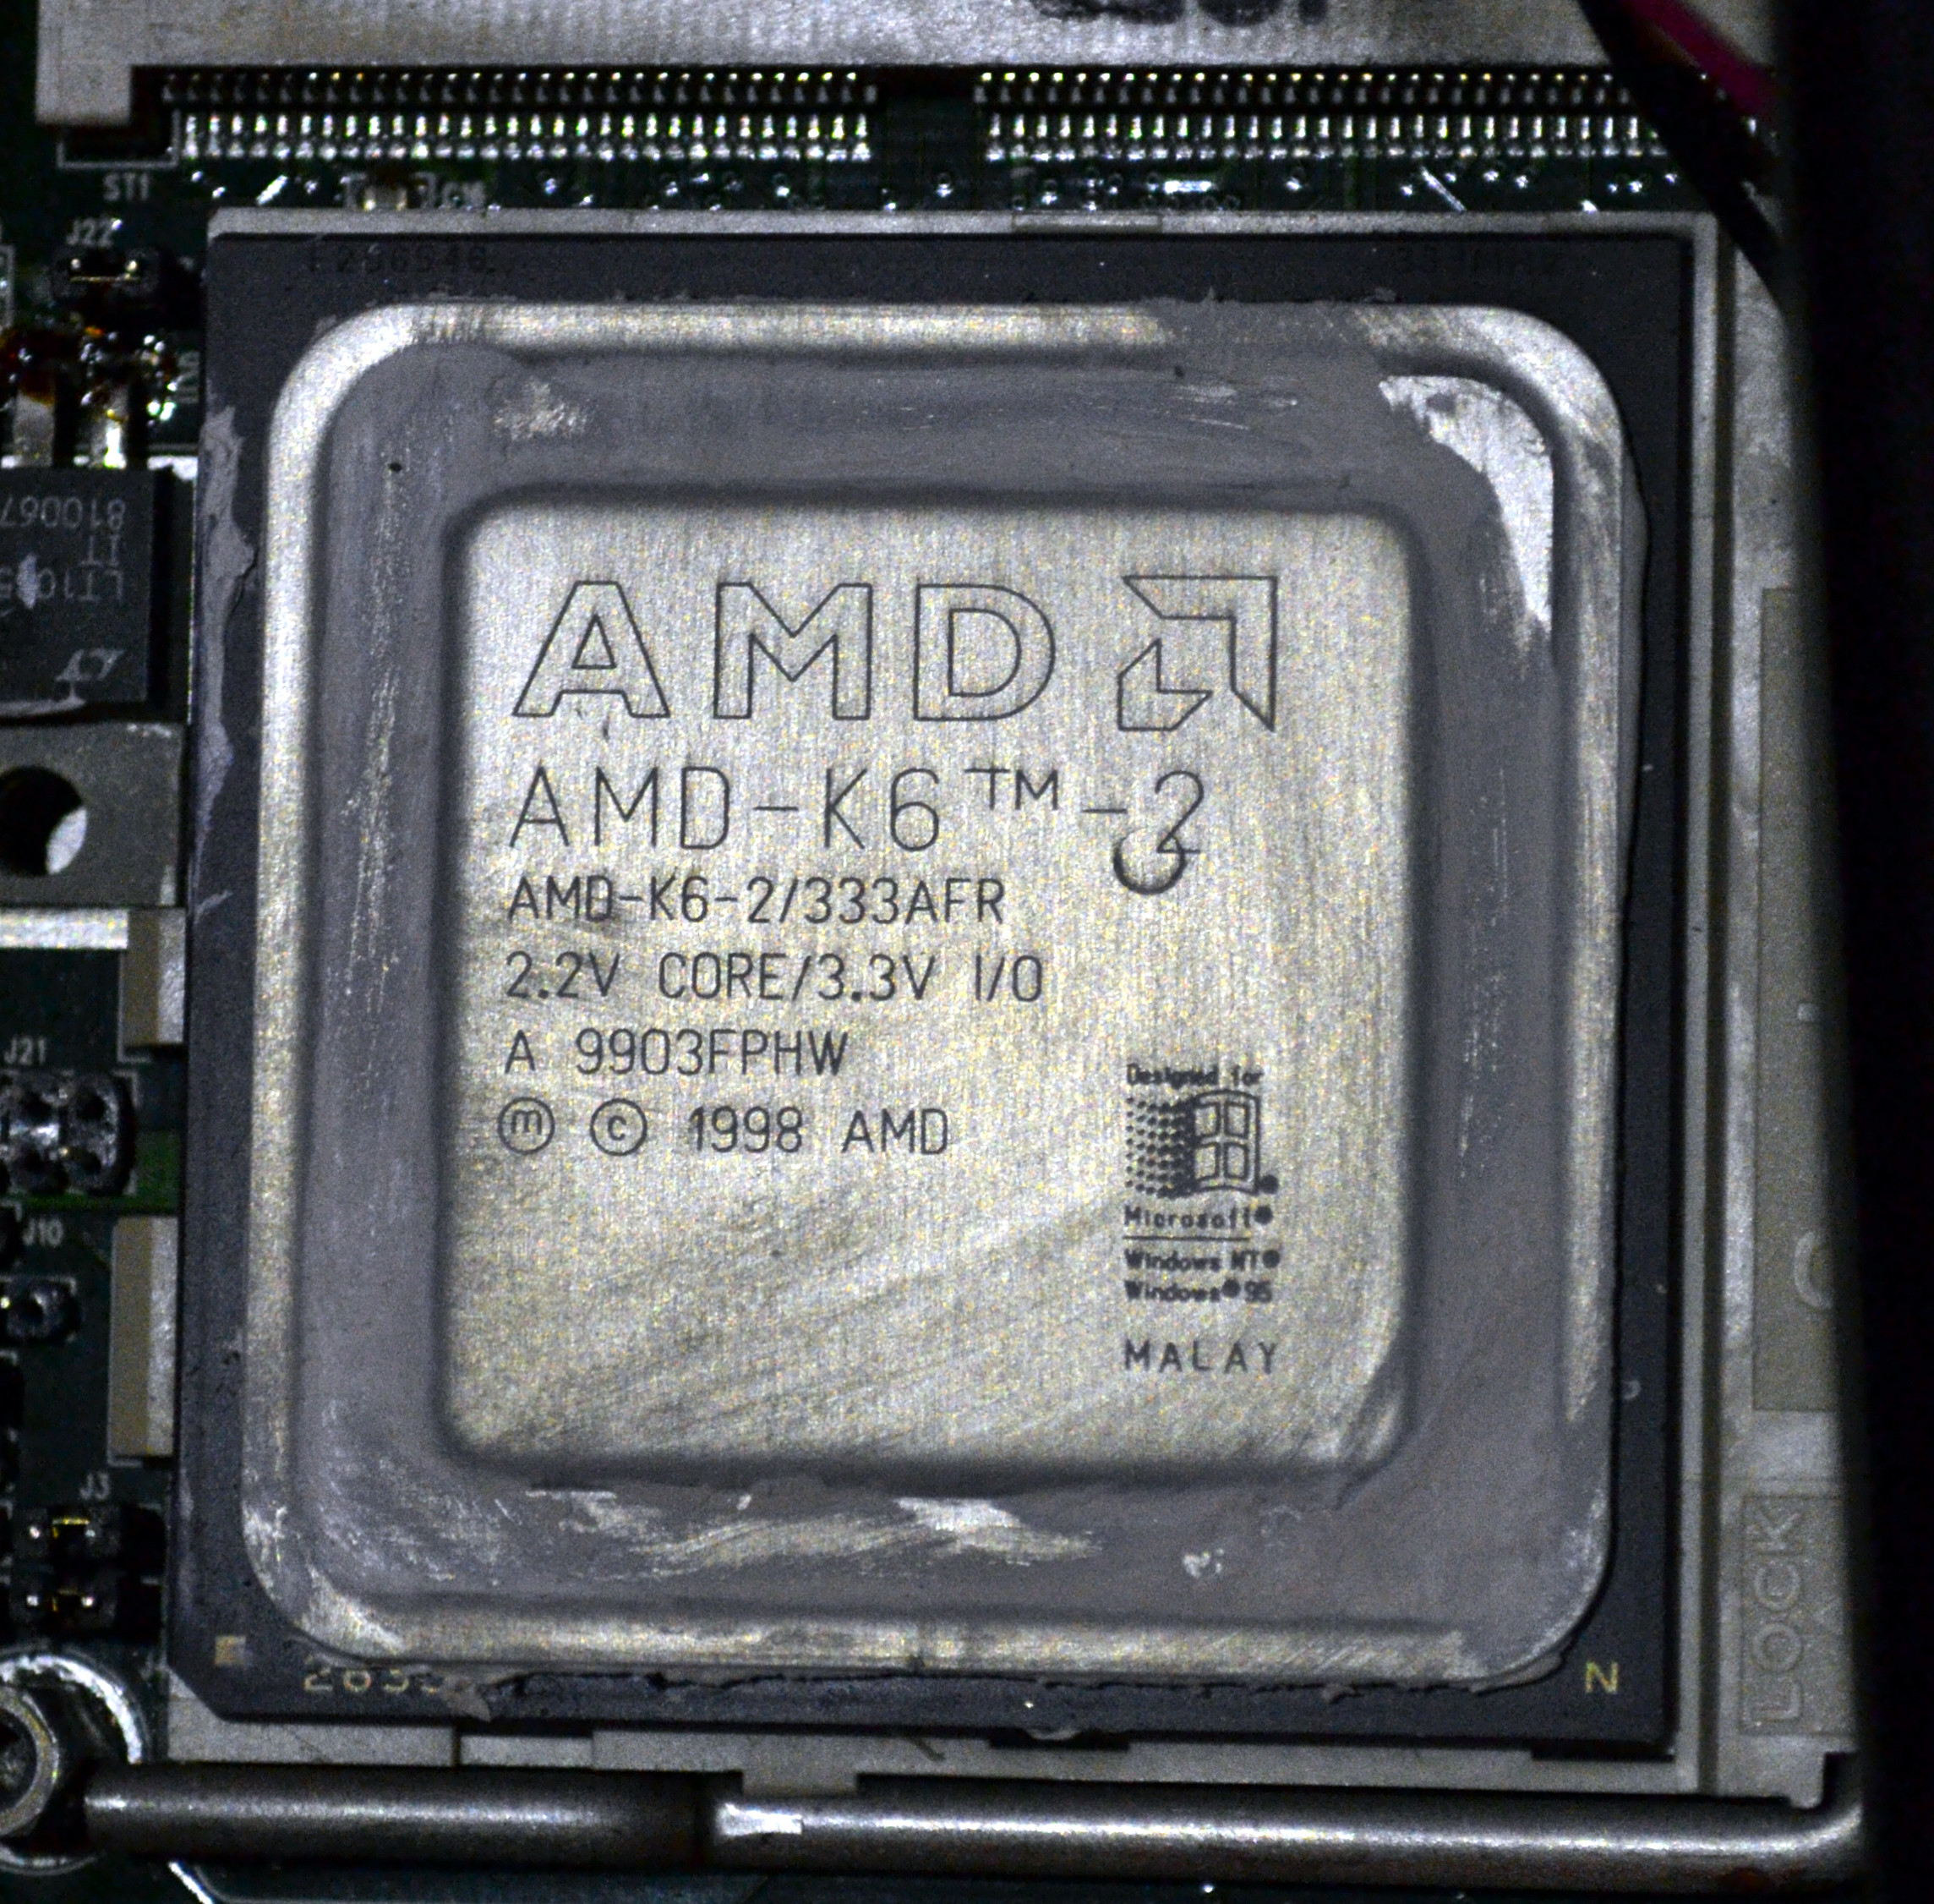
\includegraphics[width=0.500\hsize]{/home/th/repos/motonkone/pictures/processor.jpg}
\caption{AMD K6 66 MHz}
\end{figure}

\subsection{Sunit Neron liitännät}
\begin{figure}[H]
\centering
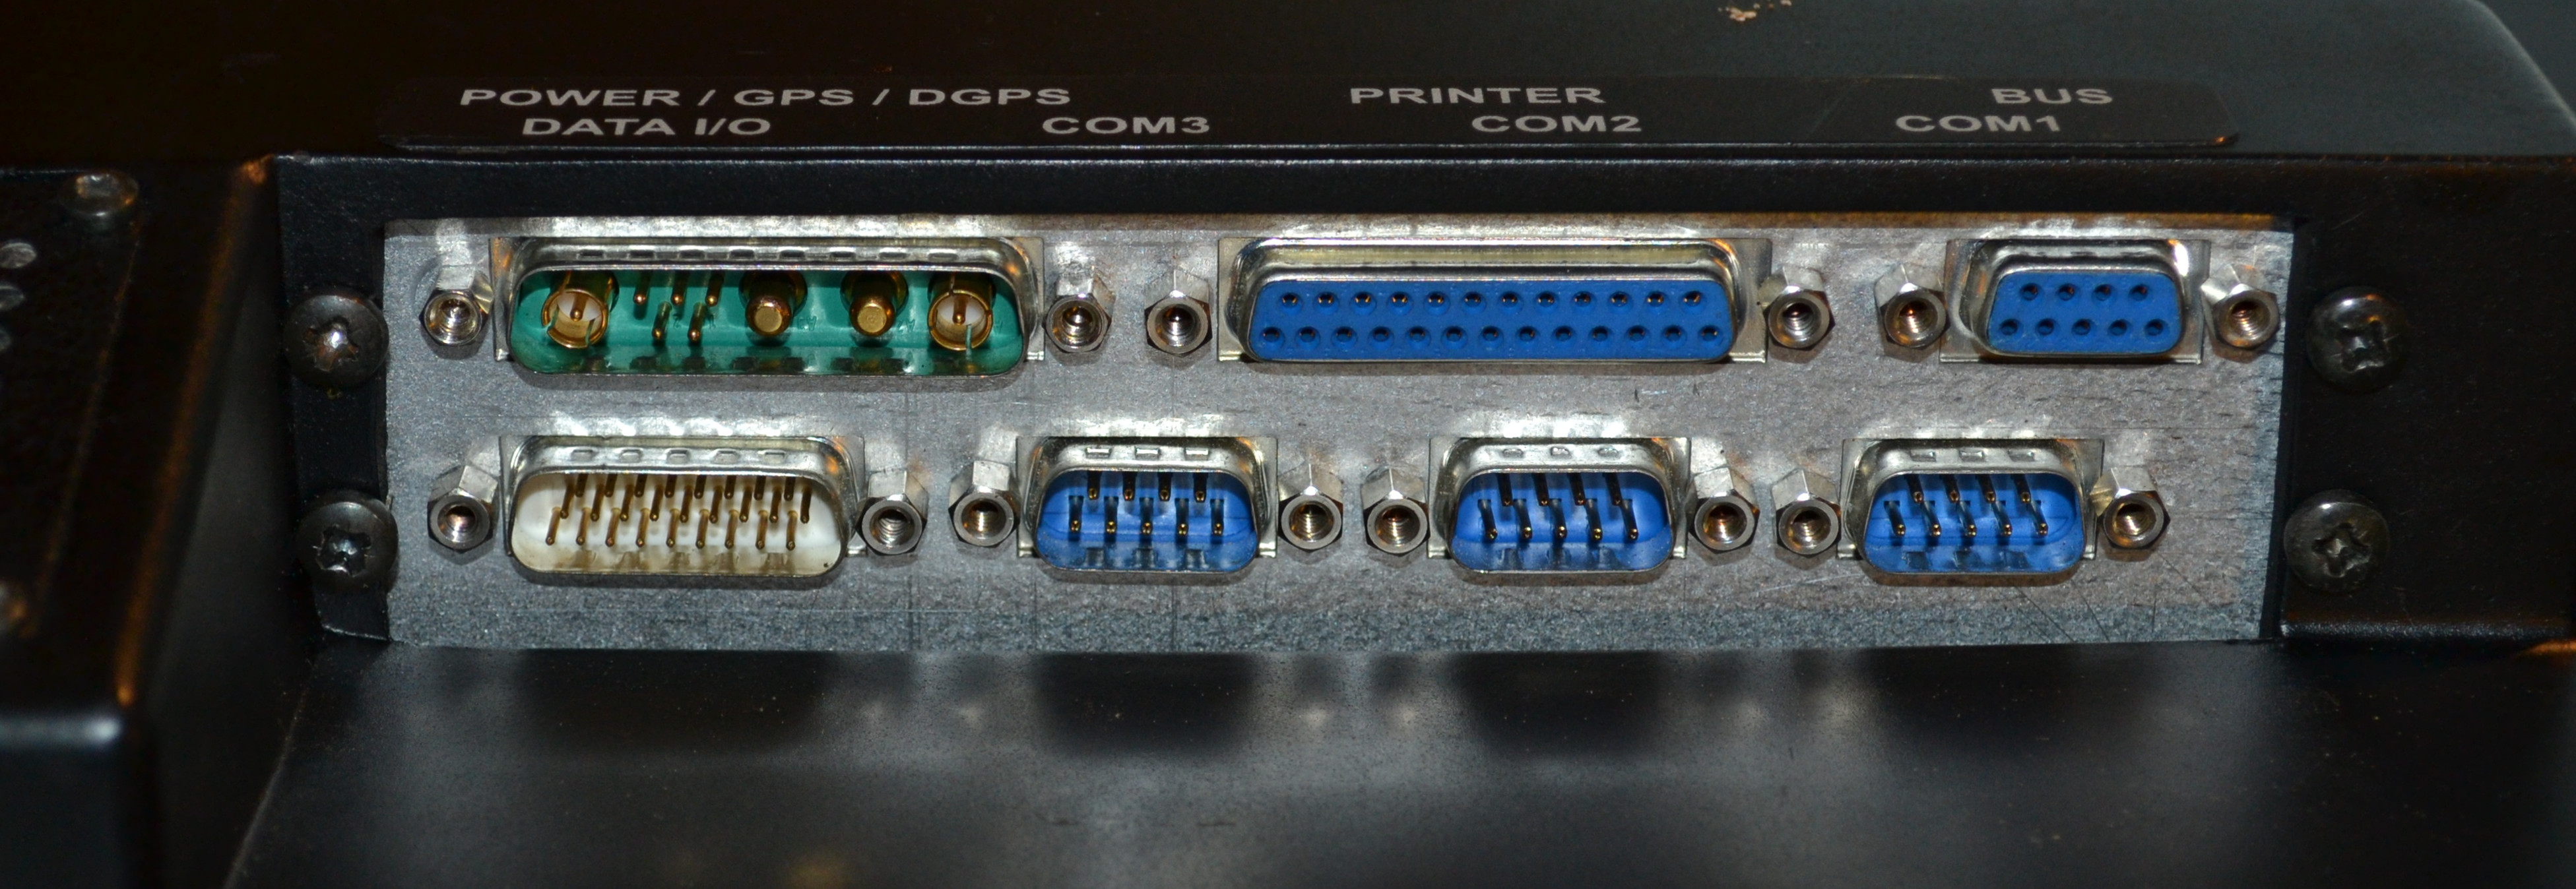
\includegraphics[width=1.00\hsize]{/home/th/repos/motonkone/pictures/sunit_nero_liitannat.jpg}
\caption{Sunit Neron liitännät}
\end{figure}

Ajoneuvotietokone Sunit Nerosta löytyy 3+1 sarjaporttiliitäntää (3x 9pin standardi RS-232, sekä yksi yhdistetty liitin), rinnakkaisporttiliitin (25pin Centronics), Sunitin oma BUS-liitin PS/2 hiirelle ja näppäimistölle, yhdistetty virta/GPRS/GPS -liitin sekä Data I/O-liitin jonka tarkoituksesta ei ole tietoa. Käytössä on kolme sarjaporttia, sekä virtaliitin. Sarjaporteista yksi on alkuperäiselle Terman-ohjaukselle, yksi Motomit IT:lle ja kolmas on luultavasti käytöstä poistettu GPS/GSM-moduuli.

\subsection{Tutustuminen Nero-ajoneuvotietokoneeseen}
\subsubsection{Ensimmäinen huolto 05/2004}
Ensimmäinen tutustuminen Sunitin Nero-ajoneuvotietokoneeseen tuli toukokuussa 2014 kun työn kohteena olevasta yksilöstä oli kiintolevy hajonnut. Tällöin tutkin ja selvitin tietokoneen ominaisuudet, liitännät ja ohjelmistot. Koska ohjelmistot oli saatavana kopioina Motomit-jälleenmyyjältä ja Valmetilta, ei alkuperäistä kiintolevyn sisältöä tarvinnut saada talteen. Tietokoneeseen hankittiin käytetty Hitachin 40Gb 2,5" IDE-kiintolevy, asennettiin käyttöjärjestelmä (Windows 98) ja ohjelmistot valmiiksi virtuaalikoneessa, varmuuskopioitiin asennus, sekä lopuksi 1.7.2014 testattiin tuotantoympäristössä että kaikki toimii oikein.

\subsubsection{Toinen huolto xx/2014}
Ensimmäisessä huollossa vaihdettu kiintolevy oli hajonnut vain muutaman kuukauden käytön jälkeen. Koska kiintolevyn koolla ja nopeudella ei ole kyseisessä tietokoneessa erityisemmin väliä, valittiin uudeksi kiintolevykorvikkeeksi paremmin tärinää ja vaihtelevia lämpö-olosuhteita kestävä SD-IDE-muistikorttiadapteri ja 2 Gb:n muistikortti. Alkuperäinen SecureDigital-standardi mahdollistaa vain 2Gb:n kapasiteetin ja väylän maksiminopeus on 12,5 Mb/s (kirjoitusnopeuden ollessa huomattavasti vähemmän, n. 1-2 Mb/s )\cite{sd:2gb}.

\subsubsection{Kolmas huolto 04/2015}
Huhtikuussa 2015 Nero-ajoneuvotietokoneesta hajosi BIOS:n CMOS-asetuksia ylläpitänyt NiMH-akku, jonka seurauksena ajoneuvotietokone kadottaa asetuksensa aina päävirtojen katkaisun yhteydessä. Kiintolevy pitää erikseen etsiä BIOS:sta, joten tämä tekee tietokoneen käytön hankalaksi tai jopa mahdottomaksi hakkuukoneen kuljettajalle. Akkupaketin NiMH-kennot uusittiin ja BIOS-asetukset määritettiin uudelleen, jolloin kone saatiin taas takaisin käyttöön.

\subsection{Valmet Terman}
Terman on Valmetin alkuperäinen DOS-pohjainen hallinta- ja apteerausohjelmisto käytettävälle hakkuukoneelle. Ohjelmiston versio on riippuvainen käytettävästä hakkuukoneesta. Kommunikointi hakkukoneen kanssa tapahtuu 9600 bitin nopeudella RS-232-sarjaporttia käyttäen. Koska mittauslaite on vaihdettu Motomit IT-järjestelmälle, käytetään Termania hakkuukoneen moottoriasetusten hallintaan.

\begin{figure}[H]
\centering
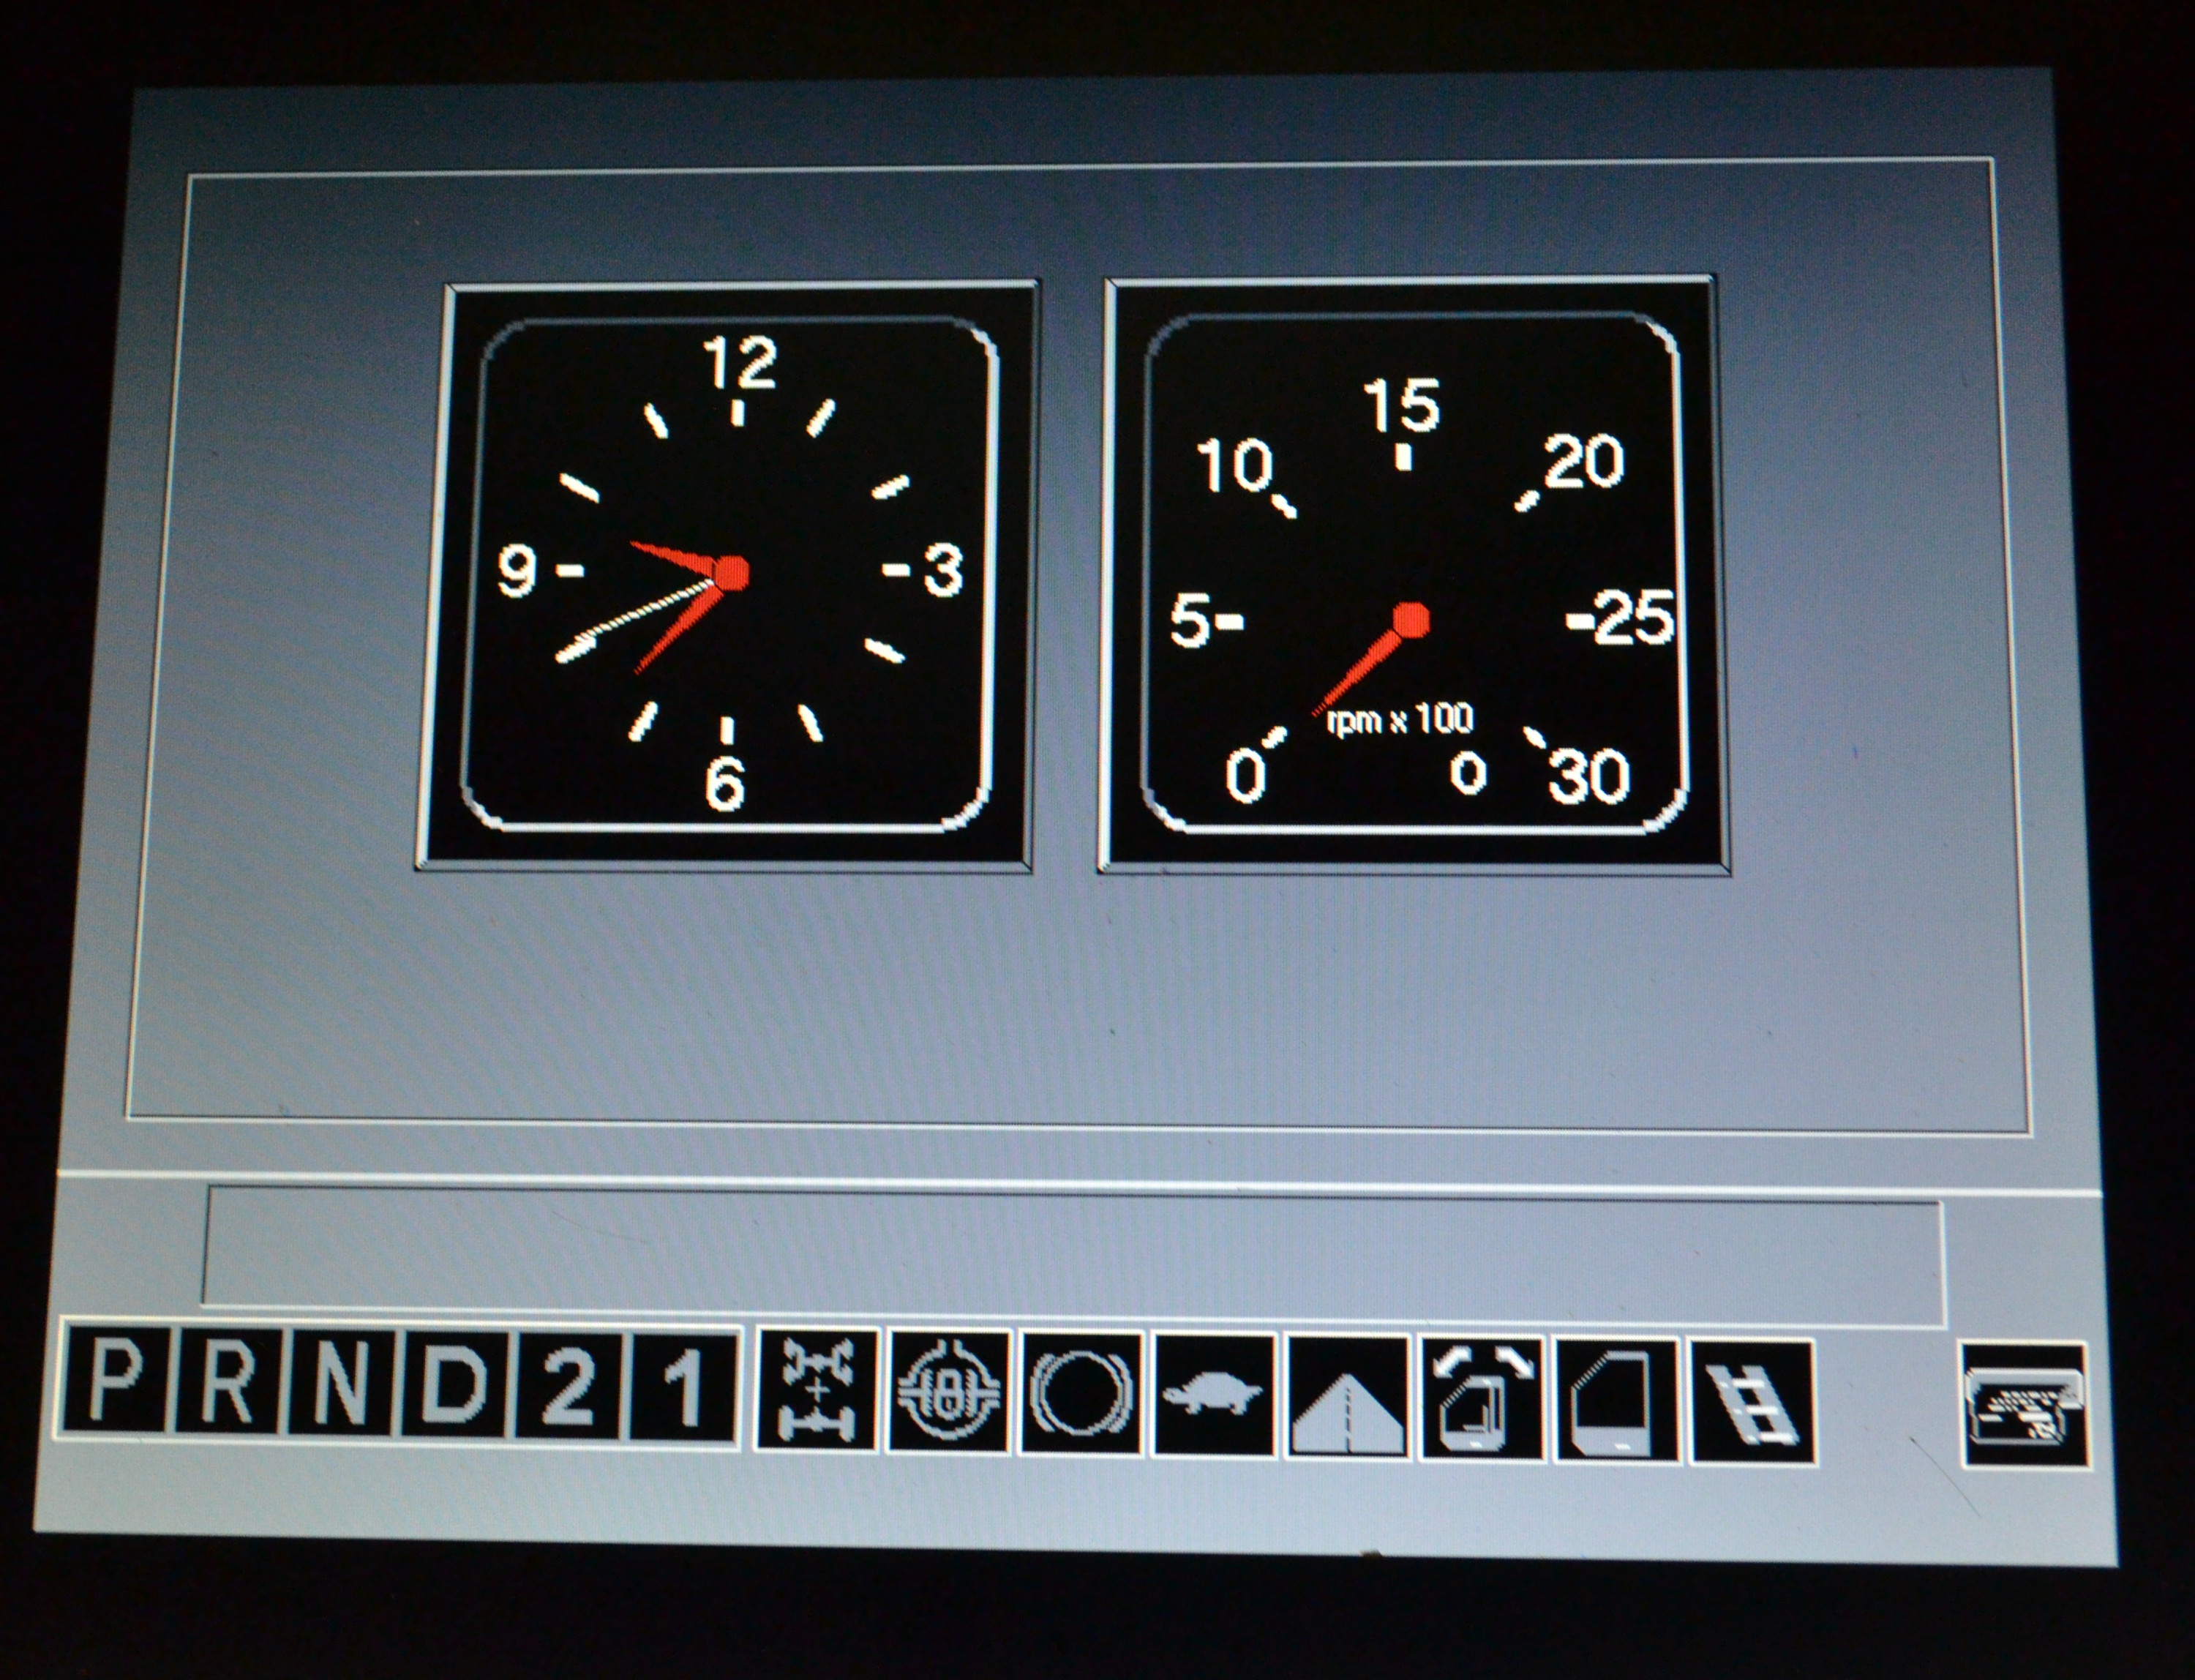
\includegraphics[width=1.00\hsize]{/home/th/repos/motonkone/pictures/terman_original.jpg}
\caption{Terman Nero-ajoneuvopc:n ruudulla}
\end{figure}

\subsection{Motomit PC}
Motomit PC on Motomit IT:n Windows-pohjainen näyttö- ja hallintaohjelmisto Motomit IT-järjestelmälle. Motomit PC kommunikoi Motomit IT:n kanssa RS-232 -sarjaväylän avulla. \cite{motomit:esite}

\begin{figure}[H]
\centering
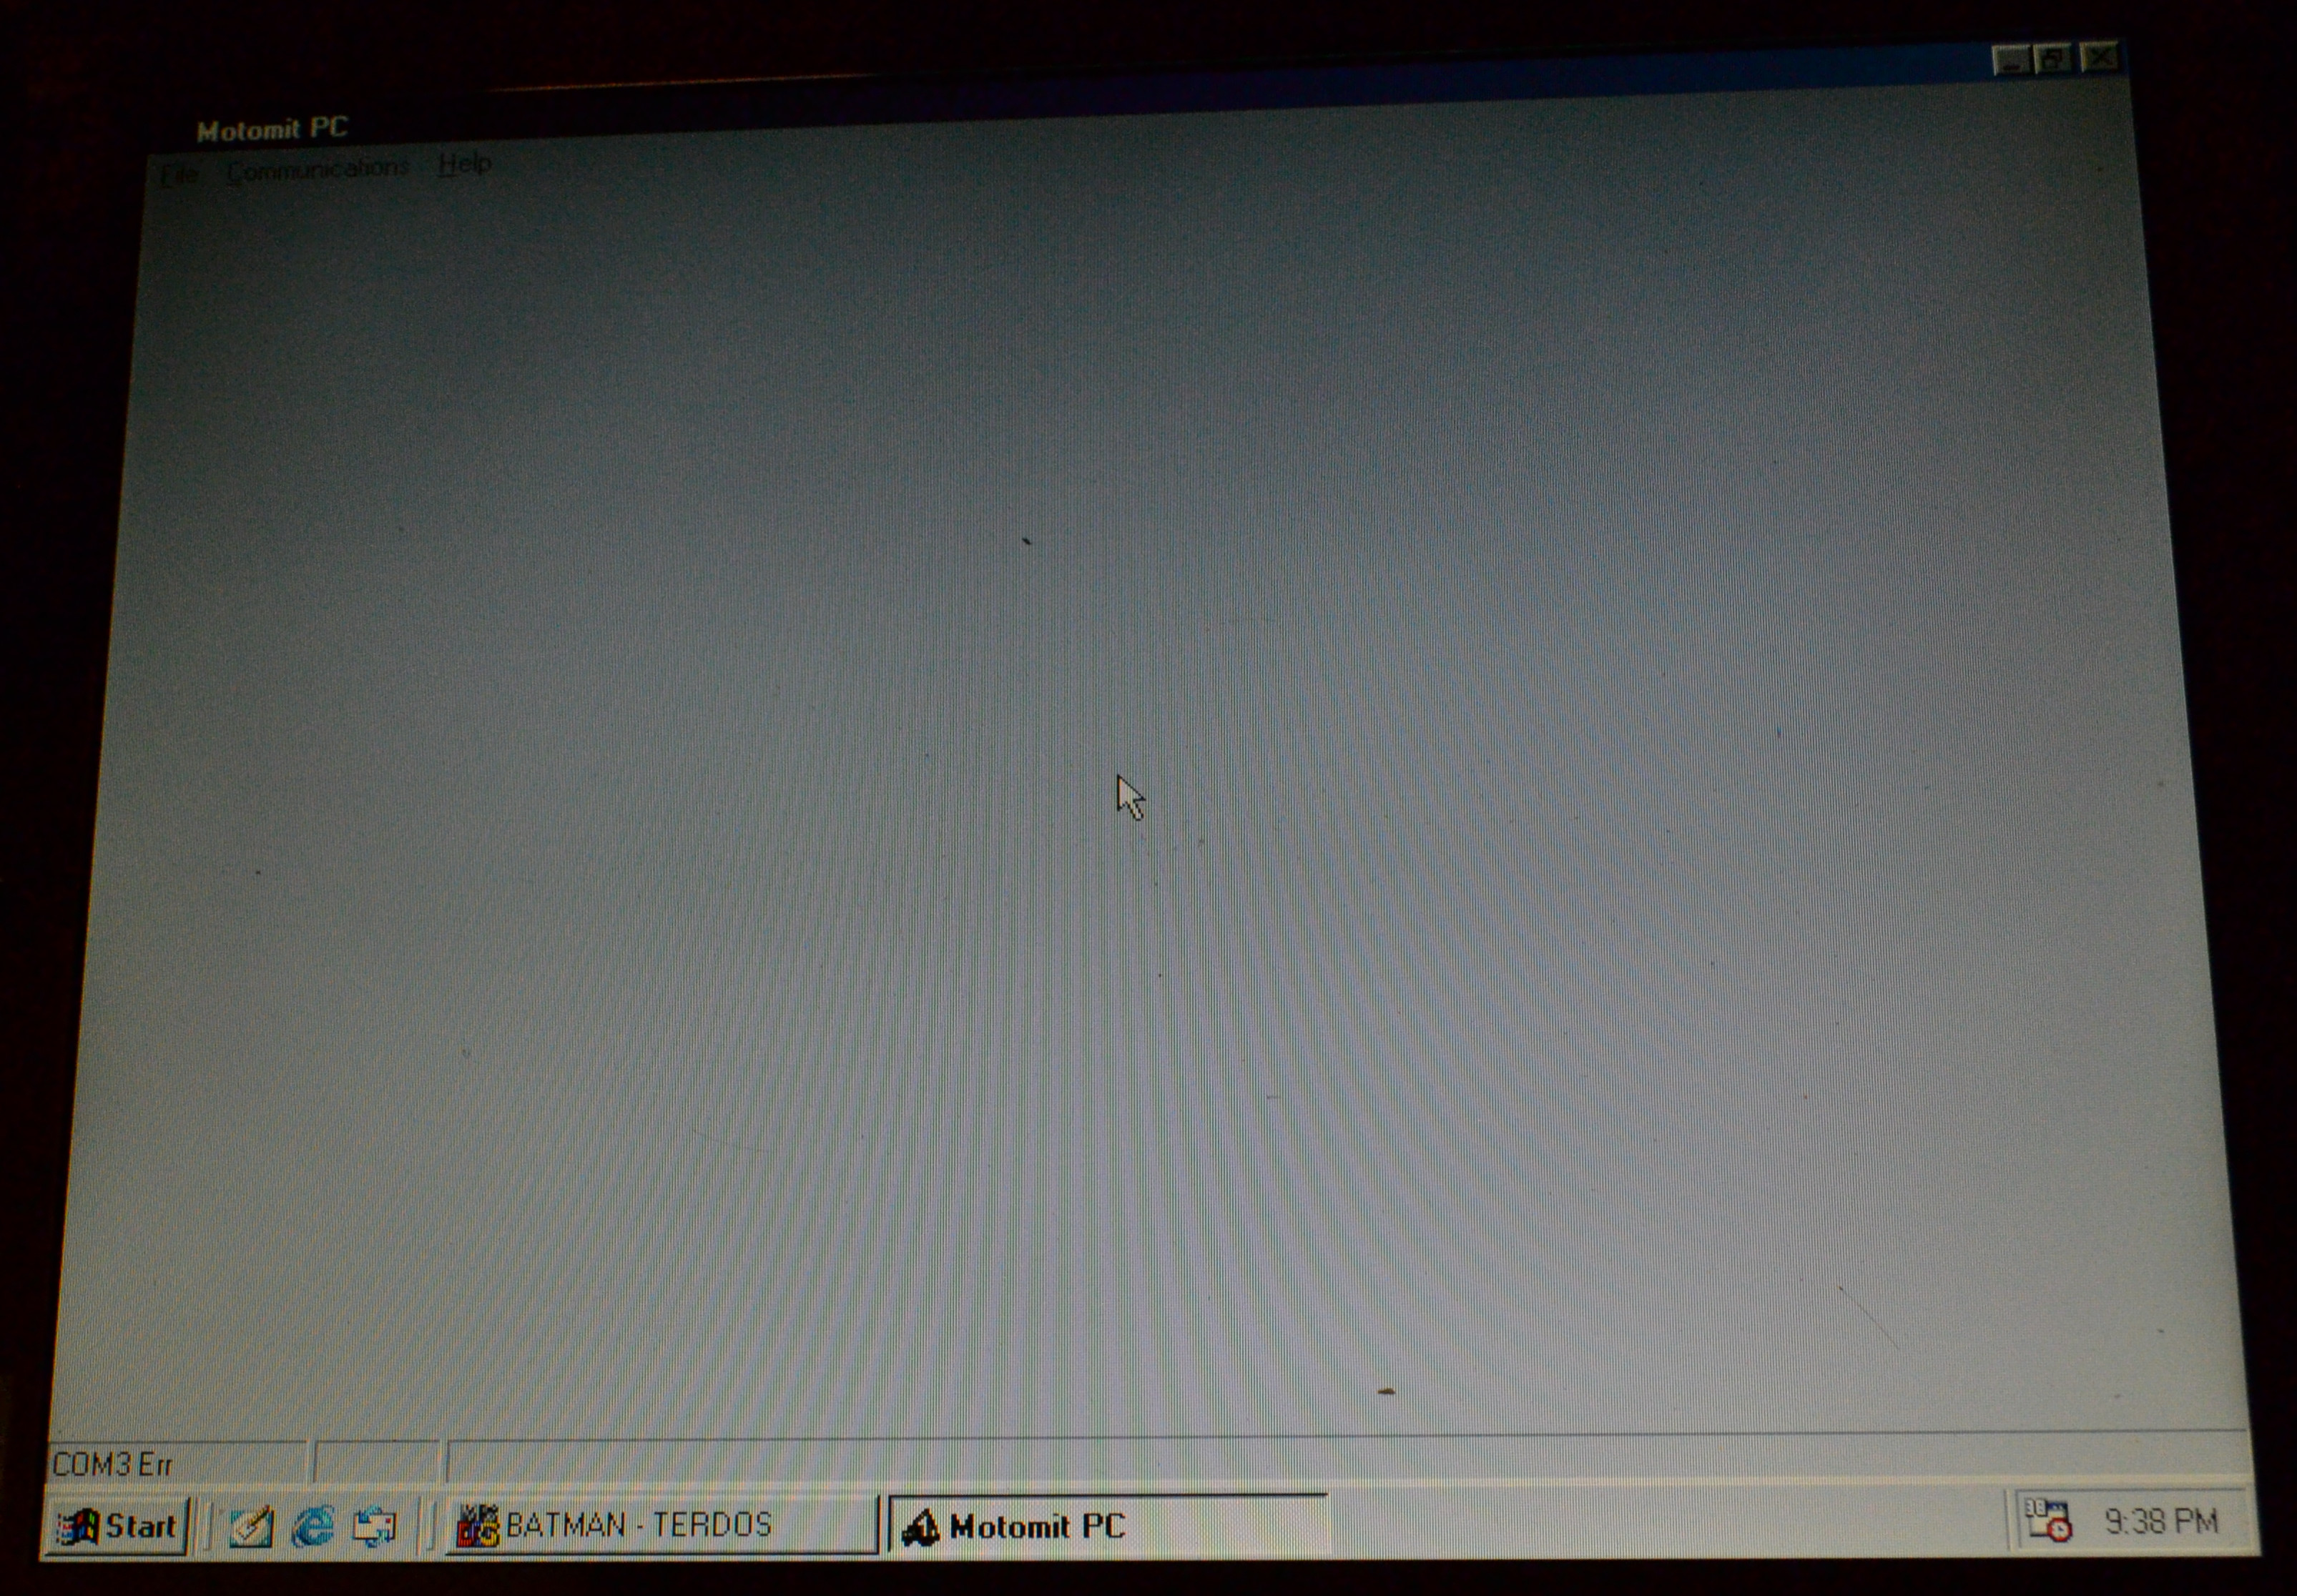
\includegraphics[width=1.00\hsize]{/home/th/repos/motonkone/pictures/motomit_original.jpg}
\caption{Motomit PC Nero-ajoneuvopc:n ruudulla}
\end{figure}

\chapter{Suunnittelu}

Jotta tietokoneen vaihto on mahdollista, tulee käytössä olevien Terman- ja Motomit PC-ohjelmistojen toimia uudessa koneessa samaan tapaan kuin vanhassa, näkyen loppukäyttäjälle (hakkuukoneen kuljettajalle) samalla tavalla kuin aiemminkin ohjelmistot ovat näkyneet.

\section{Mahdolliset toteuttamisvaihtoehdot ohjelmistojen siirrolle}

\subsection{Natiivi ympäristö}

Natiivin ympäristön vaihtoehdossa ohjelmistoja käytetään ympäristössä, johon ne on aikoinaan suunniteltu toimivaksi. Hyvänä puolena tässä vaihtoehdossa on se että ohjelmat toimivat varmasti siten kun ne on suunniteltu, mutta koska käytettävät ohjelmistot ovat vanhoja, DOS- ja Windows 98- aikaisia, niin natiivin ympärsitön käyttäminen vaatisi suunnilleen samaa ikäluokkaa olevan laitteiston käyttämisen, mitä alkuperäinenkin tietokone on. Uudemmat laitteistot eivät ole enää yhteensopivia Windows 98SE / ME:n kanssa ja lisäksi Windows 98:lla on maksimirajoituksia käytettävälle laitteistolle, kuten maksimi luotettavasti käytettävä määrä keskusmuistia on 1024 Mb ja kiintolevyosiolle on rajattu maksimikoko 127,5 Gb \cite{win98:maxspecs}. Myöskään uudemmille laitteille ei löydy välttämättä toimivia ajureita, joka rajoittaa entisestään mahdollisia laitteistovaihtoehtoja. Koska ajoneuvotietokone ei ole yhdistettynä Internetiin ja koneelle on rajattu pääsy, joten tässä käyttöympäristössä Windows 98:n paikkaamattomilla haavoittuvuuksilla (Windows 98: 84 kpl, Windows 98SE 61 kpl \cite{win98:vulns}) ei ole erityistä merkitystä käytettävyyteen.

\subsection{Ohjelmistojen rajapintojen
yhteensopivuuskerros}

Ohjelmistojen rajapintojen yhteensopivuuskerros-vaihtoehdossa  käytetään käyttöjärjestelmän ja ohjelman välissä sopivia rajapintakerroksia, jolloin saadaan käyttöjärjestelmän kanssa yhteensopimattomat ohjelmat toimimaan keskenään. Vaihtoehto vaatii yhteensopivan laitteistoarkkitehtuurin alkuperäisen järjestelmän kanssa (x86). Nykyiset Windows-versiot (Windows XP+) sisältävät jo valmiiksi yhteensopivuustilan, joka mahdollistaa vanhempien ohjelmien käyttämisen uudemmissa käyttöjärjestelmissä. Linuxissa Wine-rajapintatoteutus mahdollistaa kaikenikäisten Windows-sovellusten ajamisen Linuxissa. Myös DOS:lle löytyy rajapintakerrostoteutus Linuxiin.

\subsection{Virtualisointi}

Vaihtoehdossa alkuperäisiä ohjelmistoja+käyttöjärjestelmää ajetaan virtuaalikoneessa toisen käyttöjärjestelmän päällä. Näin saavutetaan varmin yhteensopivuus ohjelmistotasolla. Oheislaitteiden siirtämisessä virtualisoidun koneen käyttöön on rajoituksia, jotka pitää huomioida virtualisointiohjelmistoja valittaessa. Vaihtoehto kuluttaa muistia enemmän ja on hieman hitaampi kuin natiivi toteutus, hyötysuhteen ollessa \textasciitilde{}90\%  natiivista \cite{virtnat_anadtech}.

\subsection{Järjestelmäemulointi}

Vaihtoehdossa alkuperäisiä ohjelmistoja+käyttöjärjestelmä ajetaan emulaattorissa toisen järjestelmän päällä. Emuloimalla saavutetaan laitteistoarkkitehtuuririippumattomuus isäntäkoneen ja emuloitavan järjestelmän välillä. Emuloinnin haittapuolena on hitaus. Nyrkkisääntönä on 20\% hyötysuhde \cite{tinycc}, parhaat emulaattorit pääsevät n. 40-80\% hyötysuhteeseen \cite{40pperf} \cite{eltechs:exagear}

\subsection{Ohjelmistojen emulointi}

Vaihtoehdossa emuloidaan vain ohjelmat koko pc:n sijasta. Tämä onnistuu tietyillä ohjelmilla tiettyjen ohjelmistoarkkitehtuurien välillä \cite{tinycc},\cite{qemu_use}. Vaihtoehdolla voi ajaa mm. x86-ohjelmia ARM-prosessoreilla.

\section{Käytettävä toteuttamisvaihtoehto}

Tähän miksi päädyttiin x86-pohjaiseen järjestelmään, DOS-ohjelmien emuloinnilla ja Windows-ohjelmien Winettämisellä / TAI jos ei toimi niin
Virtualisoinnilla.

Raspi2+Eltechs ExaGear Desktop olisi suht. edullinen (Raspi2 35€+Exagear 30€+loput romut  \textasciitilde{}100-200€) Tee se itse-ratkaisu, mutta toimivuus olisi kyseenalainen joten todennäköisesti järkevämpää on käyttää valmiita ajoneuvopc-käyttöön tarkoitettuja x86-ratkaisuita. Kun insinöörityötä tehtiin ei Raspi2:ta ollut vielä edes julkaistu.

X86: Lorem ipsum dolor sit amet, consectetur adipiscing elit. Nunc
vestibulum magna dui, quis vestibulum libero molestie vel. Phasellus dui
risus, vehicula sit amet tincidunt nec, rutrum at erat. Aenean ex dolor,
luctus sit amet scelerisque vel, euismod vel urna. Morbi accumsan, odio
at tincidunt cursus, nibh quam consectetur turpis, at ultrices erat
lorem tristique libero. Fusce aliquet lectus sit amet sodales convallis.
Proin tempor libero eu accumsan bibendum. Proin ullamcorper tempor eros,
blandit pellentesque eros ornare vel. Nulla ac ultricies nisi. Phasellus
ligula lectus, ullamcorper in libero sit amet, pretium pretium dolor.
Nunc euismod mollis nibh, at rhoncus dolor volutpat blandit. Nam ipsum
felis, tempus ut justo ut, fringilla tincidunt augue. Vivamus non
finibus turpis, at consectetur justo.

Pellentesque ullamcorper odio at arcu venenatis consequat vel at sem.
Nulla sed scelerisque justo. Nunc consequat sem nunc, a maximus mi
ultrices non. Nunc posuere eu sapien a laoreet. Quisque sit amet mi
congue, tempus libero ut, viverra velit. Donec aliquam, metus non
rhoncus ullamcorper, magna quam pharetra lectus, in dapibus sapien
sapien quis purus. Maecenas convallis luctus semper. Nunc non ex nec est
faucibus faucibus ac eget dui. Phasellus ligula urna, lacinia in metus
nec, bibendum lobortis leo. Nunc dictum urna tortor, nec viverra dolor
suscipit et. Pellentesque vel hendrerit elit, eu pharetra quam. Cras
fringilla ullamcorper massa, quis porta justo. Praesent cursus, elit nec
finibus convallis, felis lorem luctus nulla, ut pulvinar tellus quam
feugiat turpis. Donec hendrerit massa eu ornare scelerisque. Cras non
elit vitae risus scelerisque mollis. Pellentesque vehicula sapien nec
felis eleifend blandit sit amet eu magna.

\chapter{Toteutus}

Projektissa päädyttiin käyttämään käyttöjärjestelmänä
Linux-distribuutiota Xubuntu 14.04. Alkuperäiset ohjelmistot Motomit PC
ja Terman sovitettiin käyttöön Wine-rajapinnan ja Dosbox/Dosemu
DOS-emulaattorin avulla. Järjestelmä asennettiin testausta varten
vanhaan Fujitsu-Siemensin kannettavaan. Johtuen rankoista olosuhteita,
tavallista kannettavaa käytetään vain käyttöjärjestelmän ja ohjelmien
testaamiseksi yhdessä Moton kanssa.

\section{Tarvittavat laitteistot}
\subsection{Tietokone}
Testaukseen käytetään vanhaa Fujitsu-Siemensin Amilo Pa 2510-kannettavaa vuodelta 2007. Amilo Pa 2510:ssa on AMD Turion 64 X2 TL-50 1.6 GHz prosessori, ATI Radeon Xpress X1200 128 Mb näytönohjain, 2 Gb keskusmuistia, 15.4" näyttö, sekä 120 Gb:n kiintolevy. Nämä speksit riittävät hyvin ohjelmistojen testaukseen sekä virtuaalikoneen kanssa, että emuloituna+ohjelmistorajapinnan kautta \cite{fs_amilo:review}. Puutteena kannettavassa on mm. sarjaporttien puute, sekä hajonnut näppäimistö. 

Sarjaporttiliittimet ovat poistuneet kannettavista USB:n yleistyttyä jo 2000-luvun alussa, vaikkakin vielä on myös myynnissä yrityskäyttöön kannettavia, joista löytyy vähintään yksi natiivi sarjaporttiliitin\cite{hp:laptop}. Sarjaportin puuttuminen korvataan tässä tapauksessa USB-sarjaporttiadapterilla, jonka avulla voidaan kyseistä kannettavaa tietokonetta käyttää testaukseen.

Rikkinäinen näppäimistö korvataan erillisellä USB-väylään liitettävällä näppäimistöllä testauksen ajaksi. Sähkönsyöttö testauksen ajan hoituu kannettavan omalla akulla, jossa on vielä kapasiteettia pitää kannettava käynnissä testauksen ajan / xxx h.

\subsection{USB-Sarjaportti -adapteri}
Käytettävä USB-sarjaporttiadapteri on eBaystä testaukseen hankittu 2-porttinen xxxx. 



\section{Tarvittavat ohjelmat}

Perusasennuksella asennettavaan Xubuntu-käyttöjärjestelmään tarvitsee
lisäksi asentaa seuraavat paketit, että alkuperäiset ohjelmistot saadaan
toimimaan: * Dosbox DOS-emulaattori Termania varten * Wine -rajapinta
Motomit PC:tä varten. MotomitPC tuli päivittää uusimpaan versioon, jotta
ohjelmisto toimisi winen alla.

\subsection{Xubuntu}

Xubuntu 14.04 on Ubuntu 14.04:aan perustuva (joka taas on Debianiin perustuva) Linux-distro, jossa 
käyttöliittymäksi on vaihdettu XFCE 4.10 ja mukana toimitettavista ohjelmistoista on valittu kevyemmät 
versiot kuin Ubuntussa.\cite{xubuntu:about}. Xubuntu valittiin käyttöjärjestelmäksi, koska testaamiseen 
käytettävä kannettava on 

Käyttöjärjestelmäksi valittiin Xubuntusta pitkän tuen versio 14.04.
Xubuntu asennettiin oletusasetuksilla testikoneeseen. Lisäksi Xubuntu
laitettiin kirjautumaan sisään automaattisesti, sekä Dosbox ja MotomitPC
laitettiin käynnistymään automaattisesti sisäänkirjautumisen yhteydessä.

Käytetylle USB-sarjaporttiadapterille lisättiin oma udev-sääntö, jonka
ansiosta adapterin kaksi sarjaporttia tulevat näkyviin Linuxissa
samoilla laitetiedosto (Device file)-nimillä. (ref:udev-sääntö)

\subsection{Wine}

Wine on Windows-yhteensopivuuskerros Unixin kaltaisiin (mm.
Unix/Linux/OS X/Solaris) käyttöjärjestelmiin, joka mahdollistaa
Windows-ohjelmien käyttämisen käytetyssä käyttöjärjestelmässä. Vaikka
Motomit sisältääkin taustajärjestelmänään
Linuxin\cite{motomit:manual}, niin käyttöliittymäänä tomivasta
MotomitPC -ohjelmasta on vain olemassa Windows-versio.

Jotta sarjaportit saa toimimaan Windowsin käyttämillä COM-porttinimillä
Windows-ohjelmien puolella, tulee laitetiedostoista tehdä symboliset
linkit \textasciitilde{}/.wine/dosdevices/ -hakemistoon halutuilla
nimillä (COM1 ja COM2).\cite[s. 21]{wine:manual}

\subsection{Dosbox}

Dosbox on DOS-emulaattori, joka emuloi IBM PC-yhteensopivaa tietokonetta
286/386-prosessorilla, sekä monia kyseisen aikakauden laitteistoja.
Dosbox sisältää lisäksi suoratuen sarjaportille, niin se on valittu
käytettäväksi DOS-emulaattoriksi.

Koska Dosbox on emulaattori, niin siinä pystyy säätämään
suoritusnopeutta, ruudun resoluutiota/kokoa, yms. varsin monipuolisesti.
Asetin suoritusnopeuden maksimiin, ruudun koon ikkunamoodissa kokoon
800x600 ilman näppäinlukitusta, sekä poistin ääniemulaation käytöstä.
Dosboxissa sarjaportit määritetään samasta asennustiedostosta kuin
muutkin asetukset, joten sinne piti lisätä vähintään Termanin käyttämä
sarjaportti käyttöön. (asetustiedosto
liitteenä){[}ref:http://www.dosbox.com/wiki/Dosbox.conf{]}

\section{Asennus ja asetusten säätö}
blaah. Siirrä ylempää tekstiä tänne.


\chapter{Yhteenveto}\
Tämän työn tarkoitus oli selvittää mahdolliseuudet päivittää
Moto-traktorin 20v vanha ajoneuvotietokone uudemaksi tarpeen tullessa.
Testikoneella tehdyissä testeissä alkuperäiset ohjelmistot saatiin
toimimaan uudemmissa käyttöjärjestelmissä, sekä testattua että ne
toimivat myös tuotantoympäristössä (toivottavasti). Näiden tulosten
perusteella voidaankin todeta, että alkuperäinen ajoneuvotietokone
voidaan tarpeen tullen korvata uudemmalla ajoneuvoympäristöön
tarkoitetulla laitteella kunhan uudesta laitteesta löytyy tarvittavat
liittimet (vaihtoehtoisesti vähintään 2 sarjaporttiliitäntää tai
USB-liitäntä). Nämä vaatimukset täyttyvät todennäköisesti suurimmalla
osalla tarjolla olevista vaihtoehdoista. Korvaamalla vain
laitteistopuoli ja pitämällä ohjelmat alkuperäisinä säästytään kalliilta
(ja kannattamattomalta) vaihdostyöltä, jossa kaikki kyseissen
metsätraktorin elektroniikka olisi vaihdettu uudelle ohjaukselle.

Lorem ipsum dolor sit amet, consectetuer adipiscing elit. Sed posuere interdum sem. Quisque ligula eros ullamcorper quis, lacinia quis facilisis sed sapien. Mauris varius diam vitae arcu. Sed arcu lectus auctor vitae, consectetuer et venenatis eget velit. Sed augue orci, lacinia eu tincidunt et eleifend nec lacus. Donec ultricies nisl ut felis, suspendisse potenti. Lorem ipsum ligula ut hendrerit mollis, ipsum erat vehicula risus, eu suscipit sem libero nec erat. Aliquam erat volutpat. Sed congue augue vitae neque. Nulla consectetuer porttitor pede. Fusce purus morbi tortor magna condimentum vel, placerat id blandit sit amet tortor.

Mauris sed libero. Suspendisse facilisis nulla in lacinia laoreet, lorem velit accumsan velit vel mattis libero nisl et sem. Proin interdum maecenas massa turpis sagittis in, interdum non lobortis vitae massa. Quisque purus lectus, posuere eget imperdiet nec sodales id arcu. Vestibulum elit pede dictum eu, viverra non tincidunt eu ligula.


%----------------------------------------------------------------------------------------
%   BIBLIOGRAPHY 
%----------------------------------------------------------------------------------------

\IfLanguageName{finnish}{\bibliographystyle{vancouver_fi}}{\bibliographystyle{vancouver}}
%line space
%\singlespacing %removed otherwise the appendix are also single space
\begin{flushleft}
\begin{singlespacing}
\bibliography{motonkone_biblio}
\end{singlespacing}
\end{flushleft}

%for conting the pages
\label{LastPage}~


\end{document}
